\documentclass[11pt]{article}


% --- Packages ---
\usepackage{setspace} % has to be first (for some reason)
\usepackage{amsmath, amsthm, amsfonts, amssymb, hyperref, soul, latexsym, stmaryrd, booktabs} % fonts and characters
\usepackage{enumitem, ytableau, comment, graphicx, makecell, appendix, titling, scrextend, float, subcaption, multirow, placeins, tabularray} % utilities
\usepackage{tikz, tikz-cd, tikzsymbols, pgfplots} % plots crap
\pgfplotsset{compat=1.18}
\usepackage{blkarray} % random math 
\usepackage{pstricks,pst-node,pst-tree} % networks
\usepackage{verbatim} % write code
\newlength\myverbindent % indent code
\setlength\myverbindent{0.5in} % change this to change indentation
\makeatletter
\def\verbatim@processline{%
  \hspace{\myverbindent}\the\verbatim@line\par}
\doublespacing


% --- Formatting ---
\usepackage{fullpage} % margins

\numberwithin{equation}{section} % number equations with section number
\numberwithin{figure}{section} % number figure with section number
\numberwithin{table}{section} % number table with section number

\theoremstyle{definition}
\newtheorem{theorem}{Theorem}[section]
\newtheorem{lemma}[theorem]{Lemma}
\newtheorem{claim}[theorem]{Claim}
\newtheorem{conjecture}[theorem]{Conjecture}
\newtheorem{proposition}[theorem]{Proposition}
\newtheorem{corollary}[theorem]{Corollary}
\newtheorem{problem}[theorem]{Problem}
\newtheorem{exercise}[theorem]{Exercise}
\newtheorem{definition}[theorem]{Definition}

\newenvironment{solution}{\begin{addmargin}[2em]{0em} {\bf Solution. }}{\end{addmargin}}


% --- Math Crap ---
\newcommand{\E}{\mathbb{E}}
\newcommand{\Z}{\mathbb{Z}}
\newcommand{\R}{\mathbb{R}}
\newcommand{\Q}{\mathbb{Q}}
\newcommand{\C}{\mathbb{C}}
\newcommand{\N}{\mathbb{N}}
\newcommand{\lagr}{\mathcal{L}}
\newcommand{\e}{\varepsilon}
\renewcommand{\sup}{\text{sup}}
\renewcommand{\inf}{\text{inf}}
\renewcommand{\d}{\delta}
\renewcommand{\Re}{\text{Re}}
\renewcommand{\Im}{\text{Im}}
\newcommand{\Arg}{\text{Arg}}
\newcommand{\Log}{\text{Log}}
\newcommand{\conj}{\overline}
\newcommand{\intersection}{\cap}
\newcommand{\union}{\cup}


% --- Bibliography ---
\usepackage[authordate, backend=biber, ibidtracker=false]{biblatex-chicago} % packages
\bibliography{key_bridge.bib} % .bib file


% --- Title ---
\title{Vulnerability of Urban Road Systems \\ %
    \large A Network Analysis of the Baltimore Bridge Collapse}
\author{Gavin Engelstad \thanks{Data and replication files for the document and analysis are available at \url{https://github.com/GavinEngelstad/NetSciBaltimoreBridge}. If you have questions, contact \href{mailto:gengelst@macalester.edu}{gengelst@maclester.edu}.}}
\date{Spring 2024}


% --- Document ---
\begin{document}
\maketitle

\begin{abstract}
  This paper uses network techniques, especially centrality analysis, to examine the implications of the Francis Scott Key Bridge collapse. These effects are analyzed on the road network for the entire Baltimore Metro Area using intersections as nodes and road segments as edges. We found the global network effects of the collapse were small, but that there significant local effects on the ability to traverse the network from intersections near the bridge and traffic for routes extending from the bridge. We also employ a utilization-weighted analysis to find similar but even more localized results.
\end{abstract}

\section{Introduction}

On March 26, 2024, the container ship Dali struck one of the concrete supports holding up the Francis Scott Key Bridge and caused it to collapse. The incident caused six deaths\footnote{Only four of the six bodies have been found. Still, the remaining two were on the bridge during the collapse and are presumed dead \parencite{Hassan24}.} and caused trade through the port of Baltimore, one of the largest ports in the country, to grind to a halt, costing an estimated \$15 million per day \parencites{Hassan24}{AlJazeera24}.

Pre-collapse, the Francis Scott Key Bridge was an essential part of the Baltimore road system. It was the final link in Interstate 695, or the Baltimore Beltway, a major highway that wraps around the City of Baltimore. Spanning the entire Port of Baltimore waterway, the bridge was 1.6 miles (2.6 km) across and the third-longest continuous truss bridge in the world \parencite{Parry24}. Every day, approximately 30 thousand vehicles crossed the bridge, making it an important piece of infrastructure for thousands of commuters every day \parencite{MDOT24}. Post collapse, the Maryland Department of Transportation issued a traffic warning and has observed a 7-11\% increase in traffic along alternate major highway routes across and around the port \parencites{MDOT24}{Domen24}.

This paper will examine the effects of the bridge collapse on the Baltimore Metro Area (BMA) road system using tools from complex network analysis. The rest of the paper will proceed as follows: Section \ref{sec:lit_review} will explore existing literature on the use of complex networks to analyze road network structures and robustness. Section \ref{sec:model} will outline the methods for our analysis of the effects of the bridge collapse on the road network. Section \ref{sec:data} will present the data sources that we'll use to create and examine the network. Section \ref{sec:results} will give the results to our analysis. Finally, Section \ref{sec:concl} will conclude.


\section{Literature Review} \label{sec:lit_review}

Road systems have a long history of being represented as a network. The most popular method of this, the primal approach, uses intersections as nodes and roads as links in the network \parencites{Porta06}{Ding19}. This method is seen as more comprehensive, realistic, and feasible than the alternative dual approach to modeling the network \parencites{Porta06}{Porta06b}. This approach is implemented into many software packages and databases \parencites{Esri}{Boeing17} and has the advantage that it allows for analysis that considers distance, versus solely looking at the topological properties of the network \parencites{Ding19}{Erath09}{Wang11}{Barthelemy09}.

Using this network, centrality measures can be very predictive of the real world context around roads and intersections. Typically, multiple centrality assessment (MCA) methods that analyze a number of centrality measures are used to give a comprehensive view of the network \parencites{Porta06}{Porta07}. Closeness centrality, when applied globally, is highly correlated with land-use, but fails to be meaningful looking at only a subset of a larger network \parencites{Wang11}{Porta06}{Barthelemy09}. Betweenness centrality is very effective at identifying important parts of longer routes to traverse large urban networks \parencite{Porta06}. Straightness centrality, a modification of closeness centrality where the distance along the network is divided the Euclidean distance between nodes, identifies both areas with high land-use and important routes while being robust on network subsets \parencites{Porta06}{Wang11}. Information centrality, which measures the drop in global efficiency when a piece of the network is removed, is a comprehensive measure of node importance and identifies nodes that have high centrality from all other measures \parencite{Porta06}. Eigenvector centrality is able to identify high-traffic areas and road connectivity \parencites{Jayaweera17}{Ando21}.

These tools are useful to analyze network robustness. On its own, eigenvector centrality can identify nodes in a network that are vulnerable to the removal of other nodes \parencite{Ando20}. Analysis of how stable centrality measures are when nodes are added or removed, a technique called centrality interference or centrality robustness, can act as a measure of road network robustness \parencite{Scardoni13}.

Other tools to analyze road network robustness look at the topological properties of the network after an attack, defined as the removal of edges or nodes in the network \parencite{Holme02}. The clustering coefficient, serves as a measure of reliability of a network, and how much it changes after an attack can demonstrate how the attack affects network connectivity \parencite{Xeumei10}. The change in the average shortest path also serves to demonstrate how robust people's ability to travel along the network is to an attack \parencites{Xeumei10}{Kaub24}.

This paper will implement these methods on the Baltimore road network, utilizing MCA combined with centrality interference methods along with analyzing how the average shortest path changes before versus after the bridge was destroyed. Most studies that implement these methods do so at a theoretical level and attempt to identify the edges and nodes where the network is most vulnerable to an attack \parencites{Xeumei10}{Ando21}{Masuccia16}{Julliard15}{Holme02}. The handful of studies that implement these methods that are inspired by real events tend to analyze the effects of disasters that span the entire network, like an earthquake \parencites{Kaub24}{Sakakibara04}. Therefore, this paper's application of these methods to the real-world removal of a single, important edge of a city's road network is, to my knowledge, new.


\section{Model} \label{sec:model}

\subsection{Network Structure}

The first way we'll analyze the robustness of the network is through comparing the structure of the network before versus after the destruction of the bridge.

At a global scale, that means we'll be comparing the average path between nodes. To calculate this, we'll use
\[
  \overline{d} = \frac{1}{n(n-1)} \sum_{i \in N} \sum_{j \in N, j \neq i} d_{i, j}
\]
where $N$ is the set of all nodes in the network, $n = \| N \|$ is the number of nodes in the network, and $d_{i, j}$ is the distance between nodes $i$ and $j$ traveling along the network. This will tell us how far an individual has to travel to get from one randomly chosen intersection to another. Any change in this that we observe would suggest the bridge collapse has made it harder to travel across the network. However, since the event only affected a small part of the road network, we don't expect any observed change in this to be particularly significant.

Because of this likely smaller global effect, we also want to study the local effects of the bridge collapse within the network. To do this we'll look at node level centrality measures and node-node pair level travel lengths.

For centrality measures, we'll look at the eigenvector centrality ($C^E_i$), betweenness centrality ($C^B_i$), closeness centrality ($C^C_i$), and straightness centrality ($C^S_i$). The first three of these are standard in complex network analysis and tell us whether a node is connected to important nodes ($C^E_i$), between other nodes ($C^B_i$), and close to other nodes ($C^C_i$). For $C_i^E$, we'll follow \cite{Ando20}, where roads were weighted based on capacity, and weight edges based on the type of road they represent, with highways being the highest weighted road and residential streets being the lowest weighted. For $C^B_i$ and $C^C_i$, we'll weight edges by their lengths.

Straightness centrality is a measure specific to the study of spacial networks, networks where the nodes and edges have a physical location and geographic interpretation, that tells us how directly a node can get to other nodes along the network. Introduced in \cite{Porta06}, it's calculated using 
\[
  C_i^S = \frac{1}{n-1} \sum_{j \in N, j \neq i} \frac{d_{i, j}^\text{Eucl}}{d_{i, j}}
\]
where $d_{i, j}^\text{Eucl}$ is the Euclidean distance between the points. Intuitively, a straightness centrality of 1 implies a node has a straight connection to all other nodes in the network, and anything lower tells us how inefficient traveling along the network is relative to just taking the straightest route.

To use these centrality measures to analyze robustness, we'll analyze how much they change when the Key Bridge is removed from the network. This gives us a method of assessing how individual nodes in the network were affected by the bridge collapse and where the most affected nodes are located.

To get an even more specific look at the implications of the collapse, we'll also look at how travel lengths between individual nodes are affected. To do this we'll compare $d_{i, j}$ for all $i, j \in N$ to see which routes were the most affected and what areas of the city these routes go through. This will help give us an idea of which trips the collapse will impact, and, therefore, the types of people that will be the most affected by the collapse.


\subsection{Network Utilization}

Analysis of the overall structure of the Baltimore road system will give us a general idea of how the network, nodes, and paths were affected by the bridge collapse, but it doesn't take into account how people actually use the road network. People aren't evenly spread throughout a city and equally likely start and end their journeys at all nodes.

To fix this, we'll use commute data to weight trips based on how often the routes are actually being traveled. Using this new measure, we'll look at the average shortest path length and analogues to betweenness, closeness, and straightness centrality. Because this new model changes the paths taken instead of the structure of the network, there's no useful analogue to eigenvector centrality, so that will be ignored for this portion of the analysis.

Our utilization-sensitive average shortest path length will be calculated as
\[
  \overline{d} = \frac{1}{\sum_{i \in N} \sum_{j \in N, j \neq i} n_{i, j}} \sum_{i \in N} \sum_{j \in N, j \neq i} n_{i, j} d_{i, j}
\]
where $n_{i, j}$ is the number of people traveling from node $i$ to $j$. The only addition here compared to the standard average shortest path equation is the addition of the number of people traveling the route into the sum along with a corresponding change to how we normalize the sum to account for this. 

Use-weighted betweenness centrality will be calculated as
\[
  C_i^B = \frac{1}{\sum_{j \in N, j \neq i} \sum_{k \in N, k \neq i, j} n_{j, k}} \sum_{j \in N, j \neq i} \sum_{k \in N, k \neq i, j} n_{j, k} \frac{p_{j, k} (i)}{p_{j, k}}
\]
where $p_{j, k}$ is the number of shortest paths between $j$ and $k$ and $p_{j, k} (i)$ us the number of shortest paths between $j$ and $k$ that cross $i$. Therefore, we're measuring the number of traveled paths that go through $i$, not just possible paths like with normal betweenness centrality.

Use-weighted closeness centrality will be
\[
  C_i^C = \frac{\sum_{j \in N, j \neq i} n_{i, j}}{\sum_{j \in N, j \neq i} n_{i, j} d_{i, j}}.
\]
The interpretation of this is a measure of how far individuals starting at $i$ need to travel.

Finally, use-weighted straightness centrality will be
\[
  C_i^S = \frac{1}{\sum_{j \in N, j \neq i} n_{i, j}} \sum_{j \in N, j \neq i} n_{i, j} \frac{d_{i, j}^\text{Eucl}}{d_{i, j}}.
\]
This can be interpreted as how direct the paths of individuals starting at $i$ are.

Together, this will give us tools to analyze the ways the collapse affected how people actually use the road system in the Baltimore Metro Area, not just the structure of the network like we get from the more standard estimates.


\section{Data} \label{sec:data}

For our analysis, we'll use a road network from Open Street Maps provided by the Python API from \cite{Boeing17}. This API allows us to get a directed network of roads and intersections for almost anywhere in the world, along with basic statistics about each section of road, like the exact coordinates, length, road type, and number of lanes. 

In our study, we'll focus on the 7 counties that make up the BMA: Anne Arundel, Baltimore City, Baltimore County, Carroll, Harford, Howard, and Queen Anne's County. To make our analysis both feasible and meaningful, especially when looking at eigenvector centrality and average shortest path, we exclude any intersections that aren't part of the largest strongly connected component. This results in us excluding 272 intersections in the network, mostly near the county boundaries.

The resulting network has 91,300 intersections (nodes) and 218,842 road segments (edges), 4 of which are on the Key Bridge and were affected by the collapse. A visualization of this network is shown in Figure \ref{fig:network}. We can see the road network varies substantially in node density with the densest patches near the city and to the South closer to Washington DC. The zoomed in view of the Key Bridge shows the bridge plays an unique role in the network, being the furthest east road that crosses the port. When the bridge is removed, paths that normally go across it will need to be diverted west towards downtown. Therefore, we can expect a significant number of shortest paths to be rerouted and affected.

\begin{figure}[t]
	\caption{Baltimore Metro Area Road Network}
  \begin{subfigure}{0.49\textwidth}
    \centering
    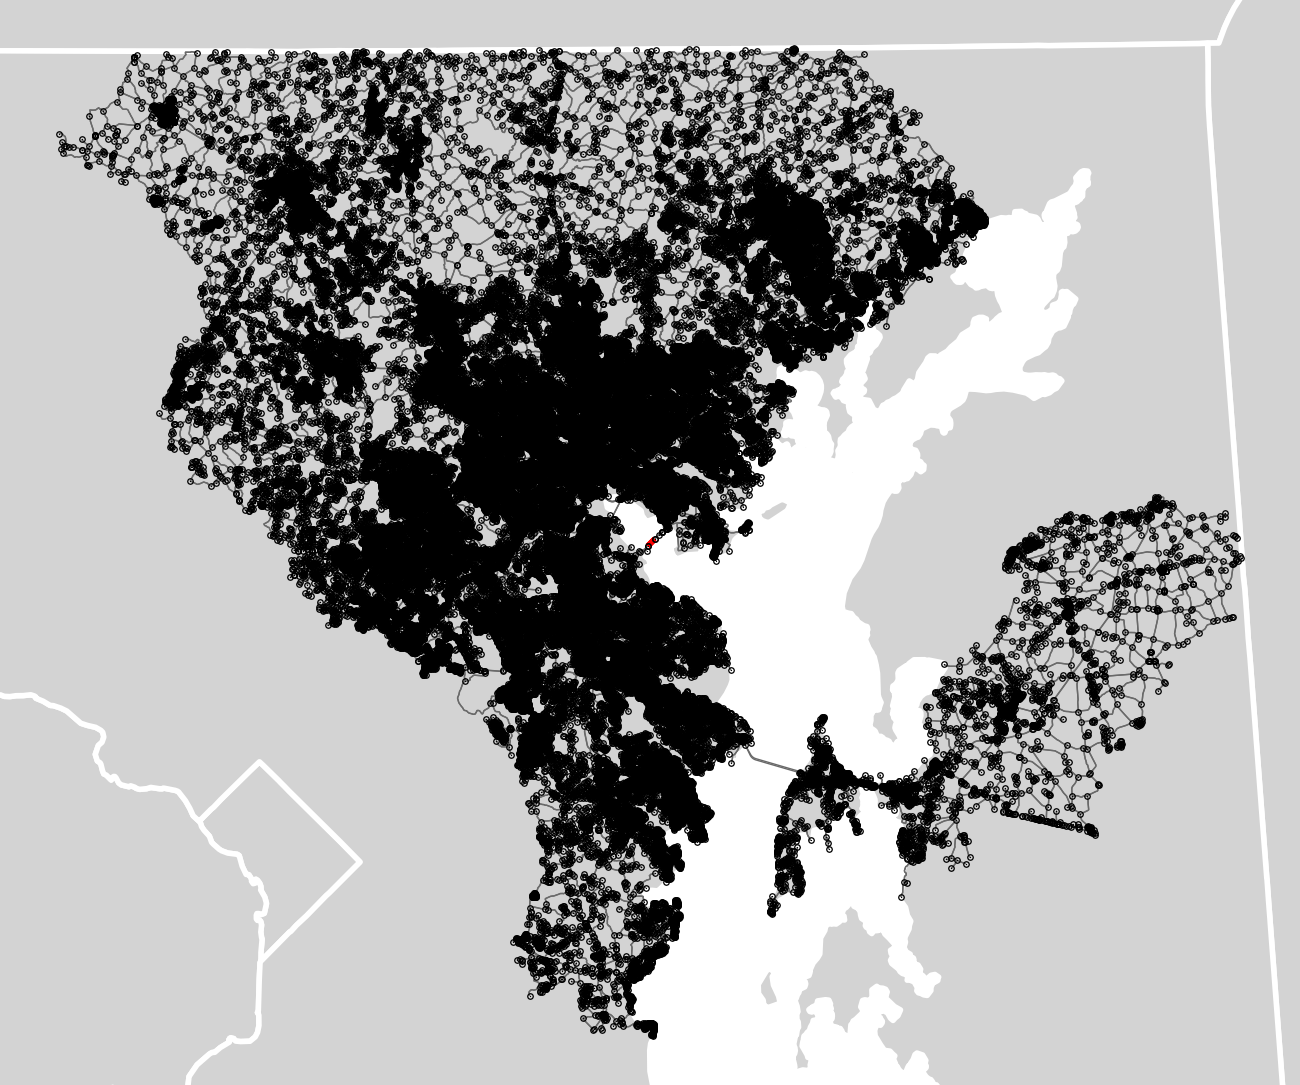
\includegraphics[width=\textwidth]{maps/full_network.png}
    \caption{Total BMA Network}
  \end{subfigure}
  \begin{subfigure}{0.49\textwidth}
    \centering
    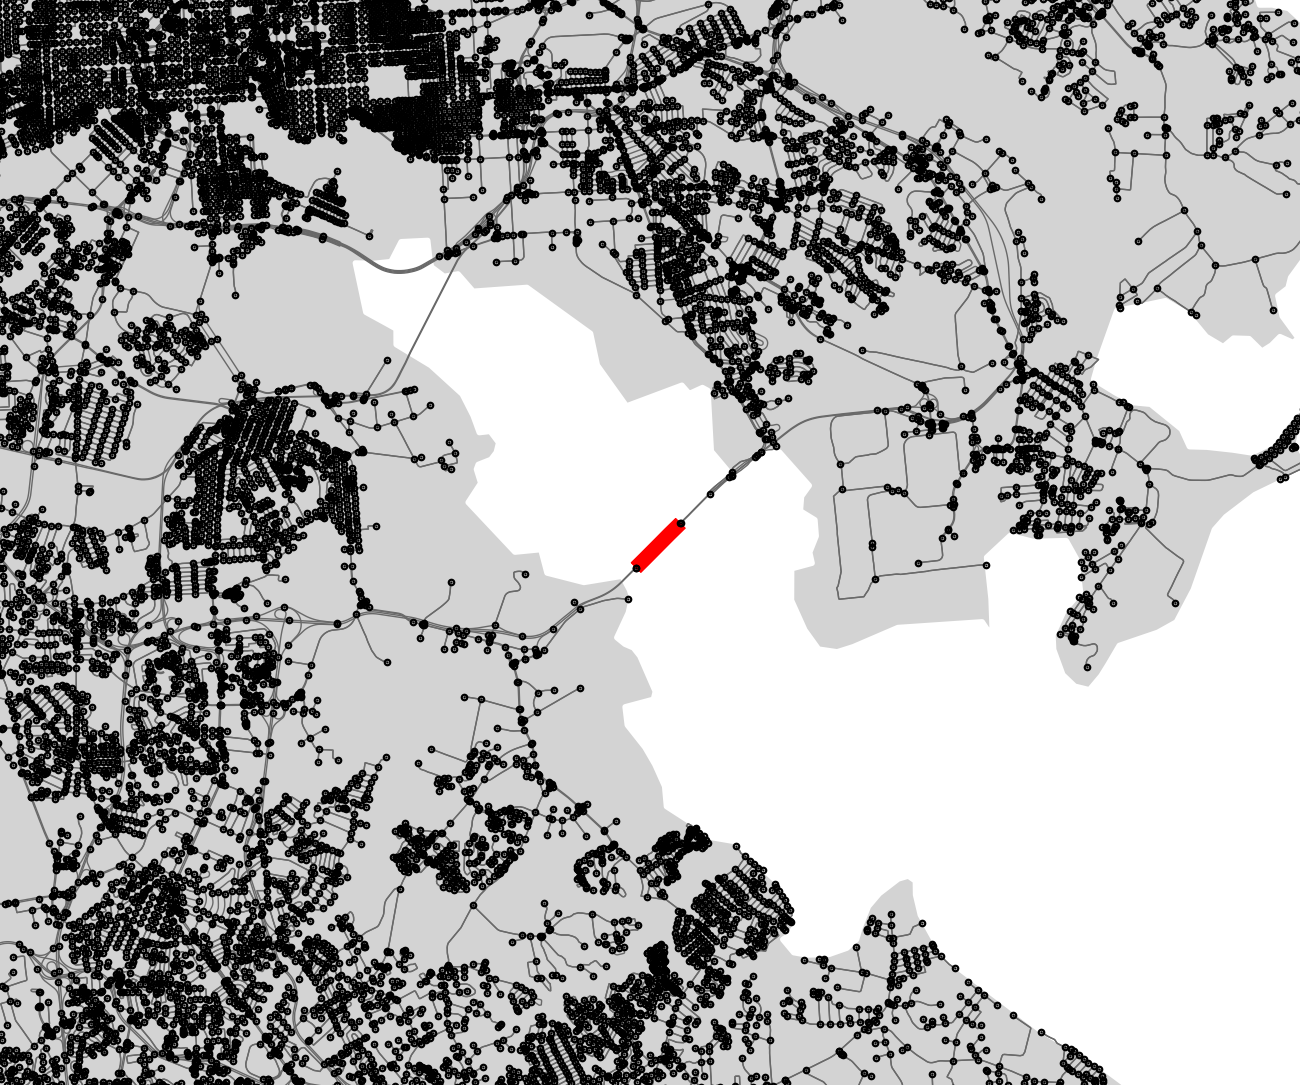
\includegraphics[width=\textwidth]{maps/zoomed_network.png}
    \caption{Zoomed In to Key Bridge}
  \end{subfigure}

  \begin{center}
    {\footnotesize \emph{Note:} Key Bridge highlighted in red.}
  \end{center}
  \label{fig:network}
\end{figure}

For data on network utilization, we'll use census tract level journey-to-work flows from the US CENSUS \parencite{Bolton20}. This data gives bilateral flow estimates for the number of daily commuters from each census tract to every other census tract from 2012 to 2016. This isn't the time period we're interested in, but is the most recent data available. Due to the bounds of the road network we're working with, we only include commuters who both live and work within the BMA. This excludes 11.1\% of commuters who work in the BMA and 12.2\% of commuters who live in the BMA.

The dataset includes 678 tracts within the BMA. 672 of these are home to at least one commuter and all 678 are the workplace of at least one commuter. Together, there are 41,272 residence-workplace pairs which 1.02 million commuters travel between. The maps in Figure \ref{fig:tracts} shows the commuter volume into and from census tracts in the BMA. We can see that commuter residences are somewhat evenly distributed throughout the area, but workplaces are much more centralized. When we calculate paths commuters are taking along the network, this will mean that the paths will point to a much more central location, which may limit how many go across the Key Bridge. The density plot in Figure \ref{fig:tracts} shows that commuter flow has a significant right-skew which even appears on a log-scale plot. This means that commuter flows are, typically, fairly low, but there are tract pairs with much higher flow.

\begin{figure}[t!]
	\caption{Baltimore Metro Area Census Tracts by Commuter Volume and Flow}
  \begin{subfigure}{0.49\textwidth}
    \centering
    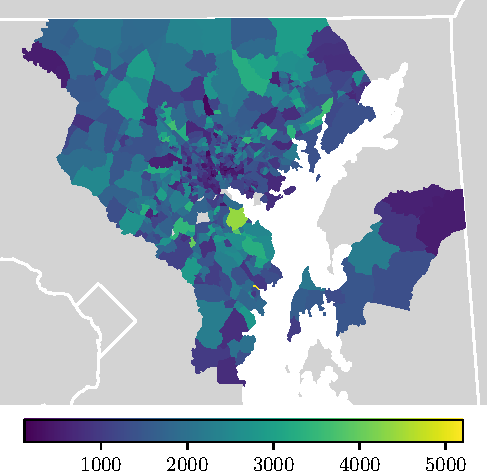
\includegraphics[width=\textwidth]{maps/tract_home.pdf}
    \caption{Commuter Residences in Tract}
  \end{subfigure}
  \begin{subfigure}{0.49\textwidth}
    \centering
    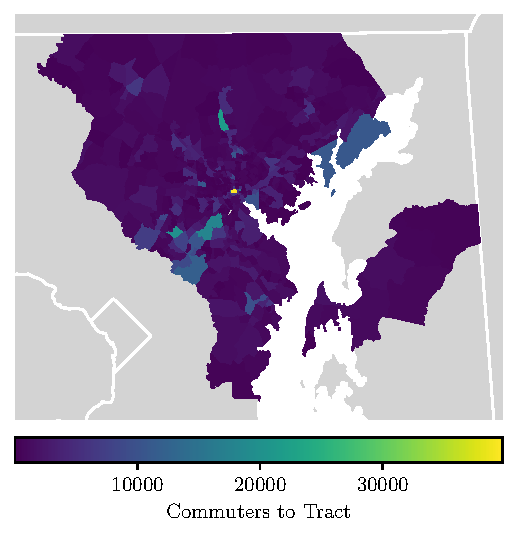
\includegraphics[width=\textwidth]{maps/tract_work.pdf}
    \caption{Commuter Workplaces in Tract}
  \end{subfigure}
  \begin{subfigure}{\textwidth}
    \centering
    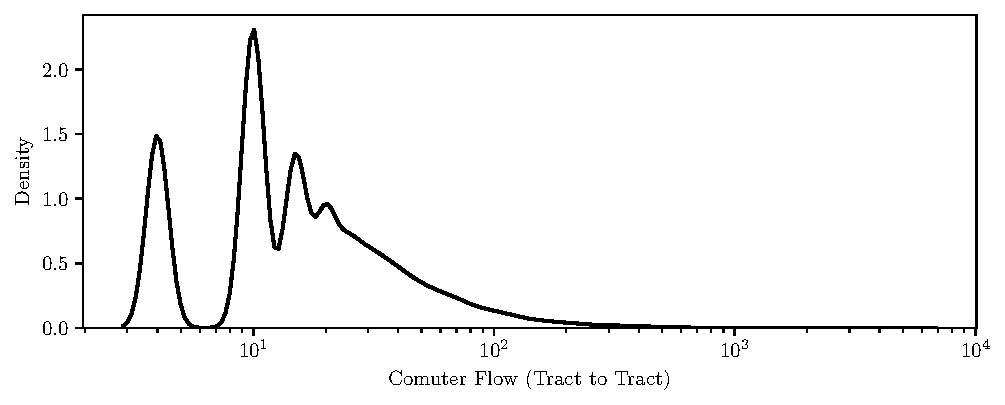
\includegraphics[width=\textwidth]{graphs/tract_flows.pdf}
    \caption{Tract to Tract Bilateral Commuter Flows}
  \end{subfigure}

  \label{fig:tracts}
\end{figure}

We are limited by the granularity of this data. Census tracts are very large compared to the intersection/road segment scale of the network, which means we can't perfectly estimate the paths commuters are taking.\footnote{From a data protection and privacy standpoint, especially in a public dataset, this limitation is very reasonable.} In our analysis, we'll estimate paths with commuters starting and ending at the intersection closest to the center-of-mass of the census tracts they're traveling between and assuming all commuters travel along the road network. This should give us a reasonably accurate estimate for how commuters are traveling, although will have some errors, especially closer to the center of mass for the higher-volume census tracts.


\section{Results} \label{sec:results}

\subsection{Network Structure}

The average shortest path length along the network is 26.3 miles (42.3 km) with the bridge and 26.4 miles (42.5 km) without the bridge. That means the destruction of the bridge increased the average shortest path length by 0.09 miles (0.14 km). This difference of only 0.003\% of the pre-collapse average shortest path is relatively small, and suggests the network-wide implications of the event were minimal.

At a node level, Figure \ref{fig:cents} shows the calculated centralities for intersections in the BMA with the bridge, without the bridge, and the difference between the two.


\begin{figure}[t!]
  \caption{Node centrality before and after the bridge collapse.}
  \centering
  \resizebox{.96\textwidth}{!}{% <------ Don't forget this %
    \begin{tblr}{%
      colspec = {cX[c,h]X[c,h]X[c,h]},
      rowsep = 0pt,
      colsep = 4pt
      }
      & \textbf{Network With Bridge} & \textbf{Network Without Bridge} & \textbf{Difference} \\
      $C^E_i$ & 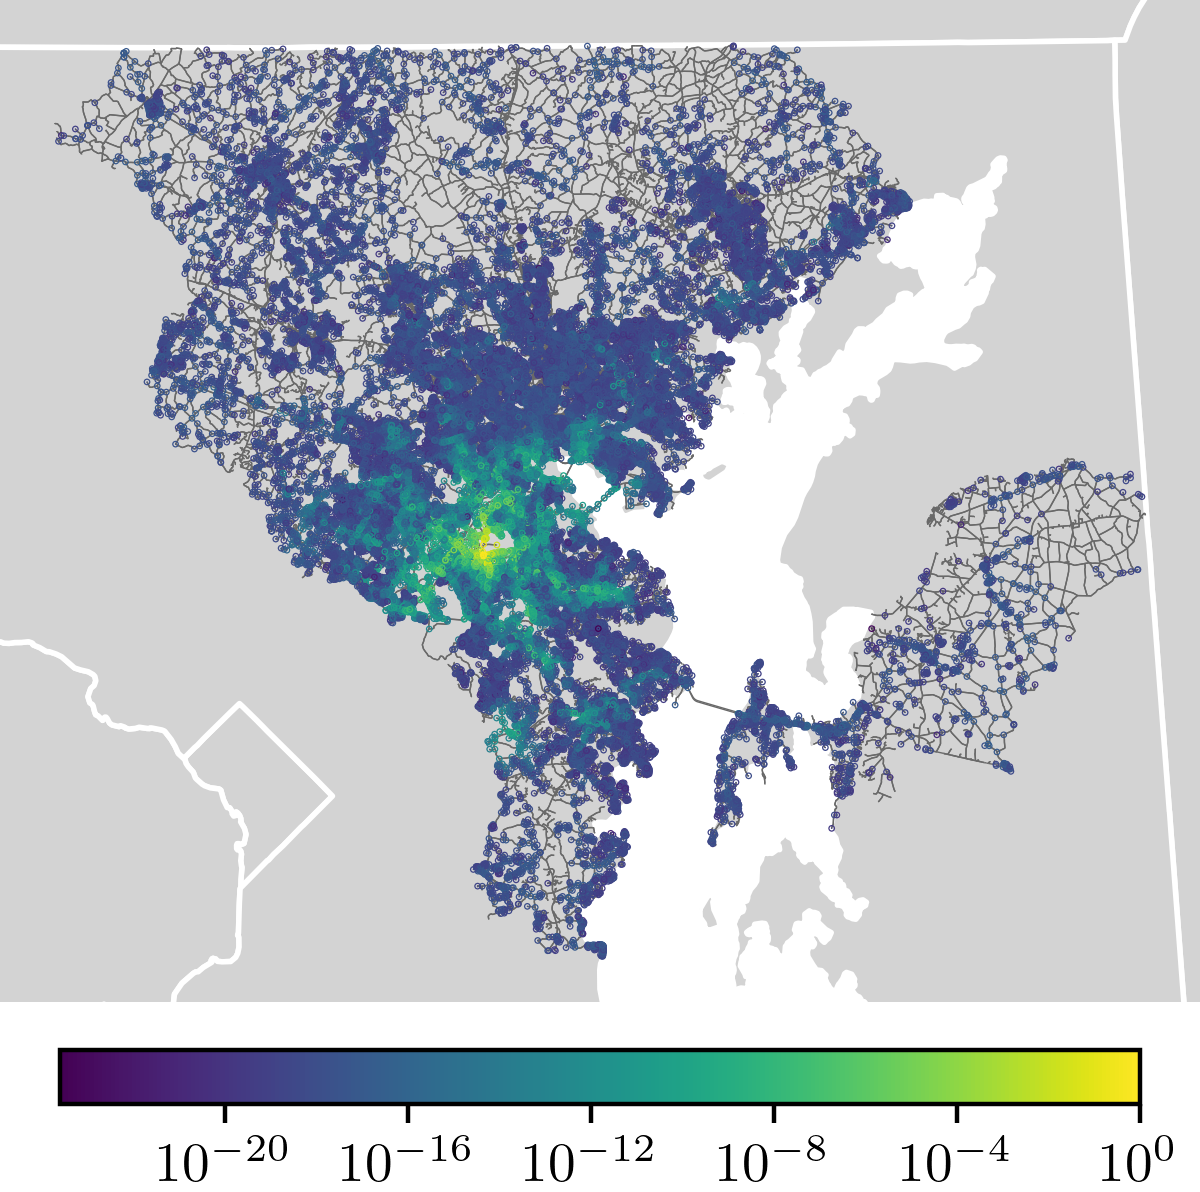
\includegraphics[width=0.28\textwidth]{maps/eigenvector_w_bridge.png} & 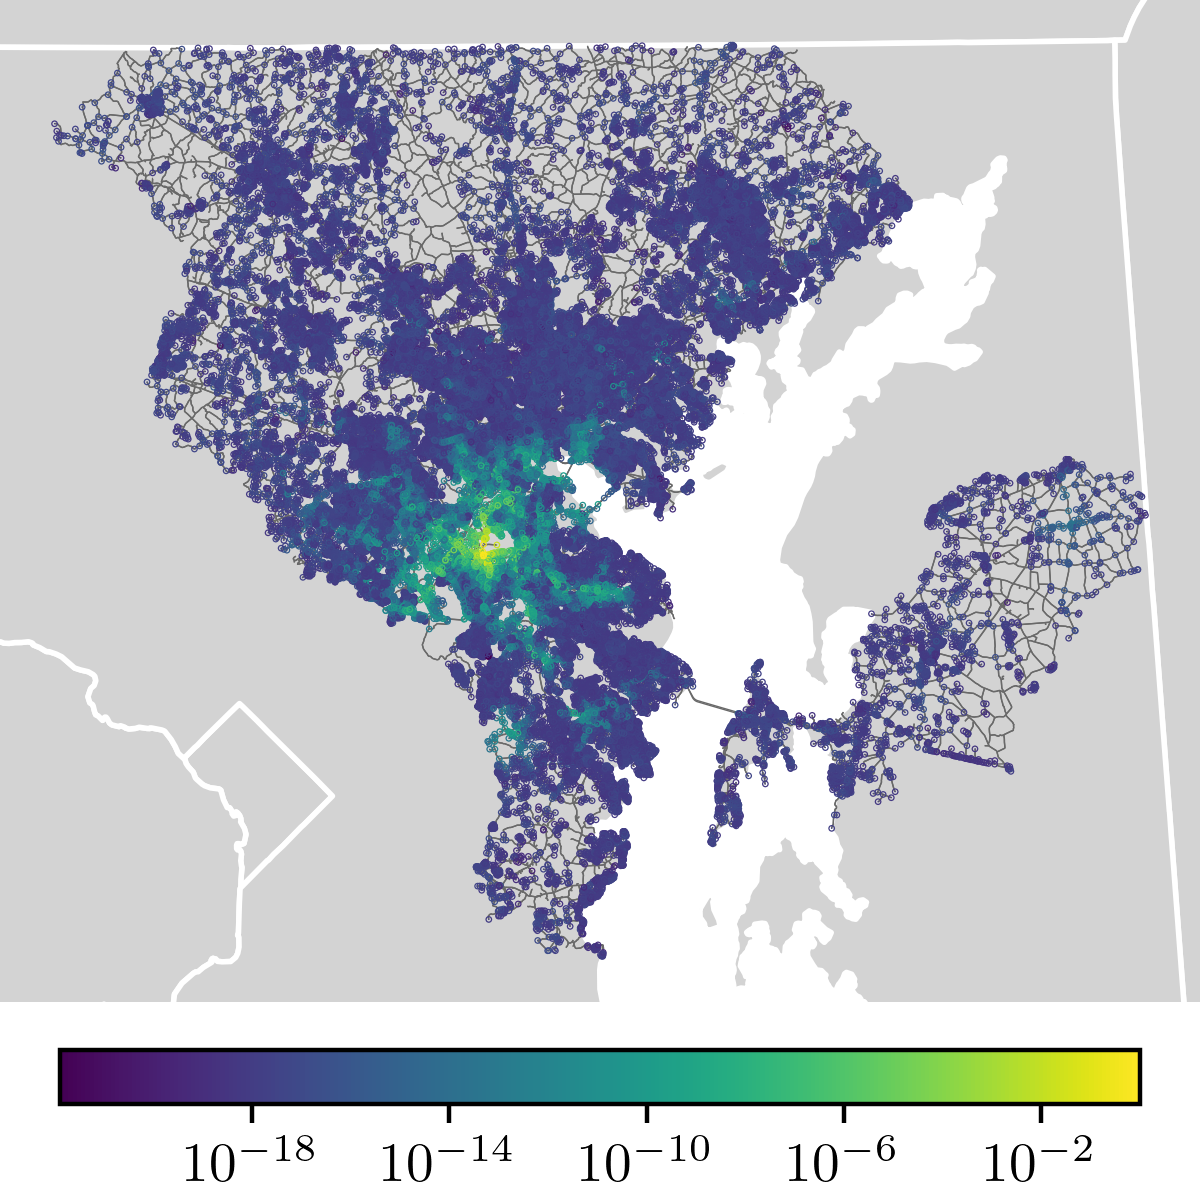
\includegraphics[width=0.28\textwidth]{maps/eigenvector_wo_bridge.png} & 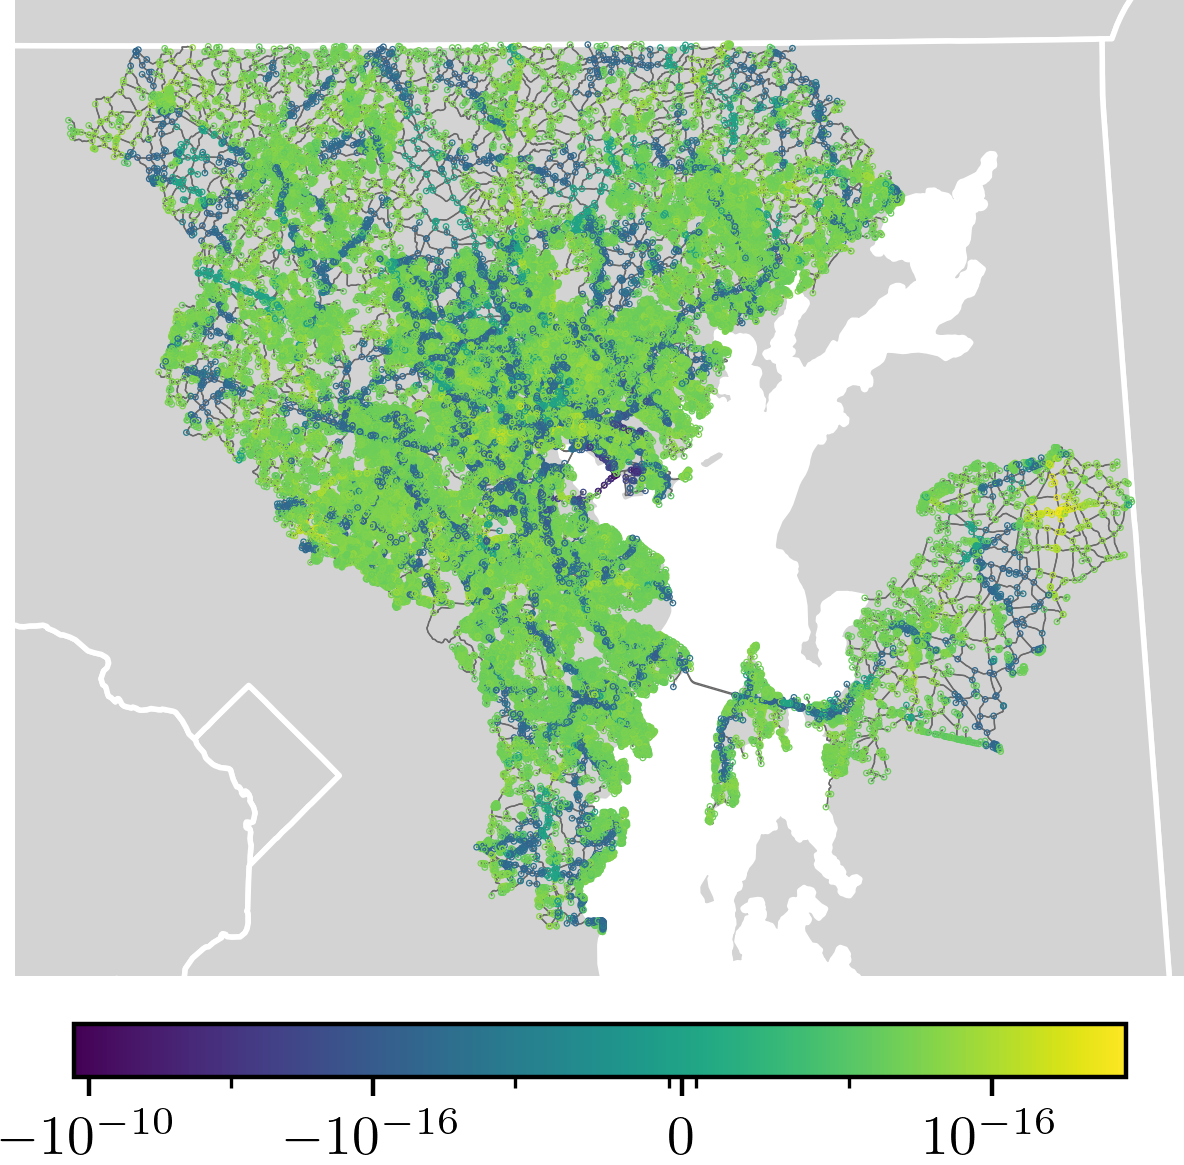
\includegraphics[width=0.28\textwidth]{maps/eigenvector_diff.png} \\
      $C^B_i$ & 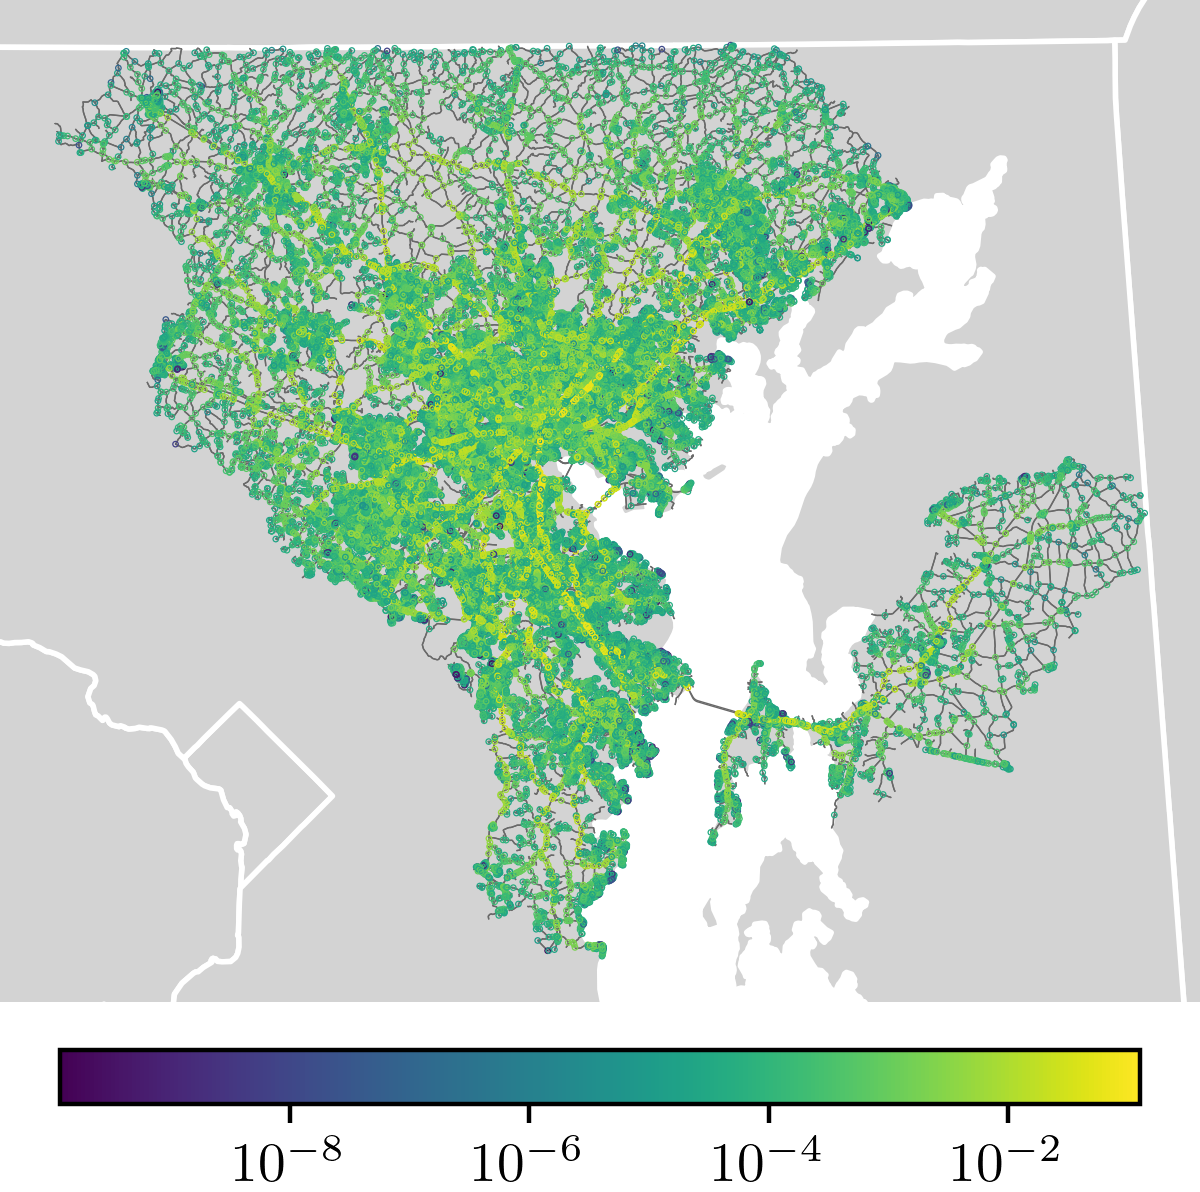
\includegraphics[width=0.28\textwidth]{maps/betweenness_w_bridge.png} & 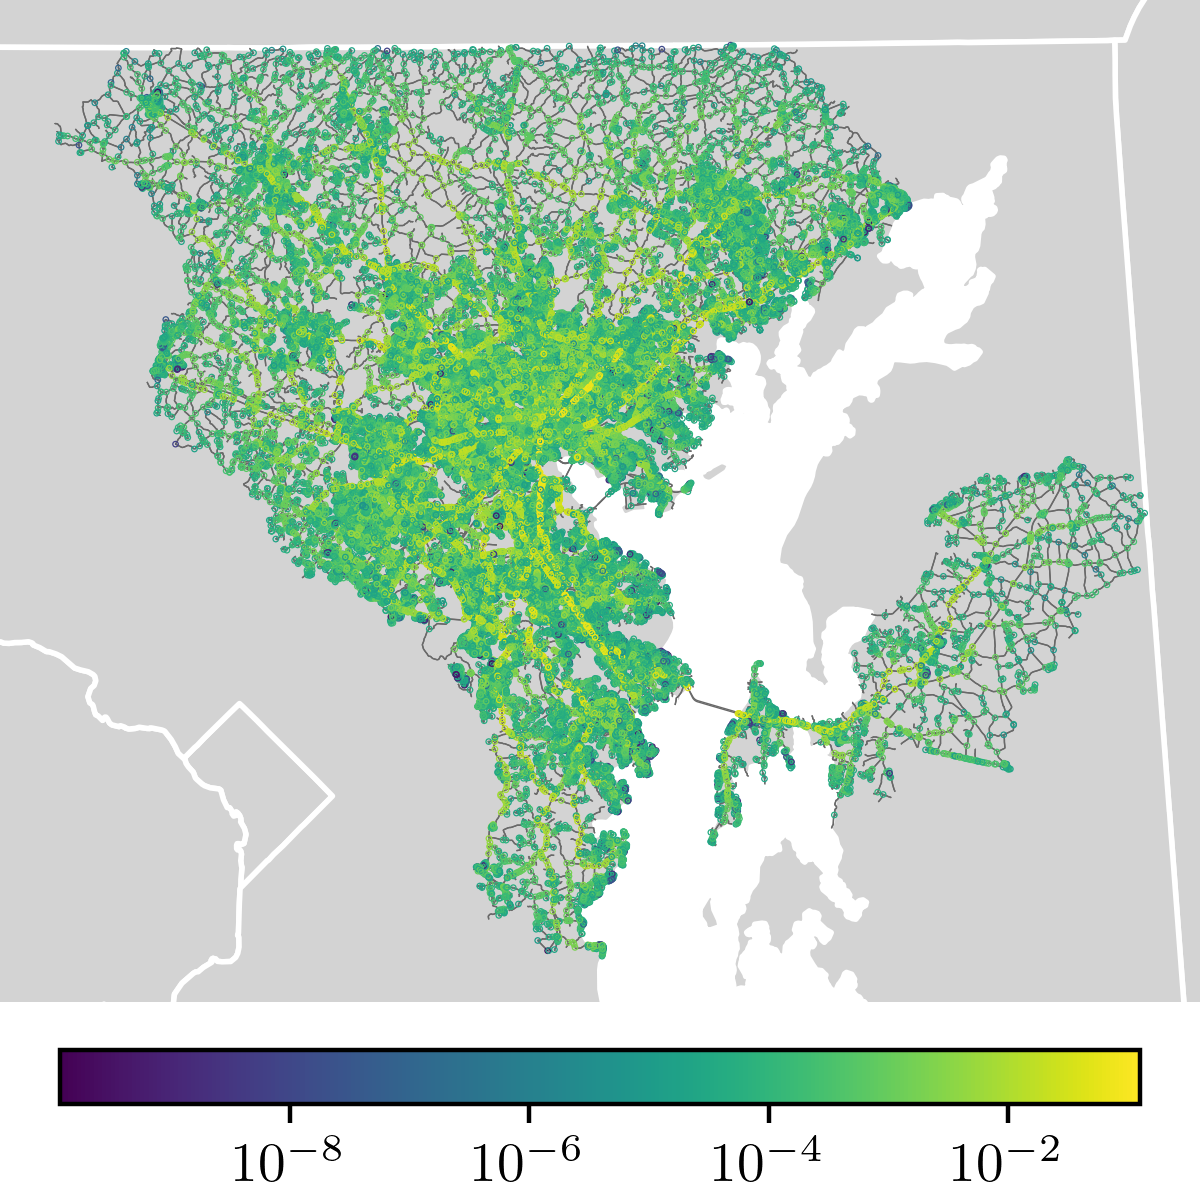
\includegraphics[width=0.28\textwidth]{maps/betweenness_wo_bridge.png} & 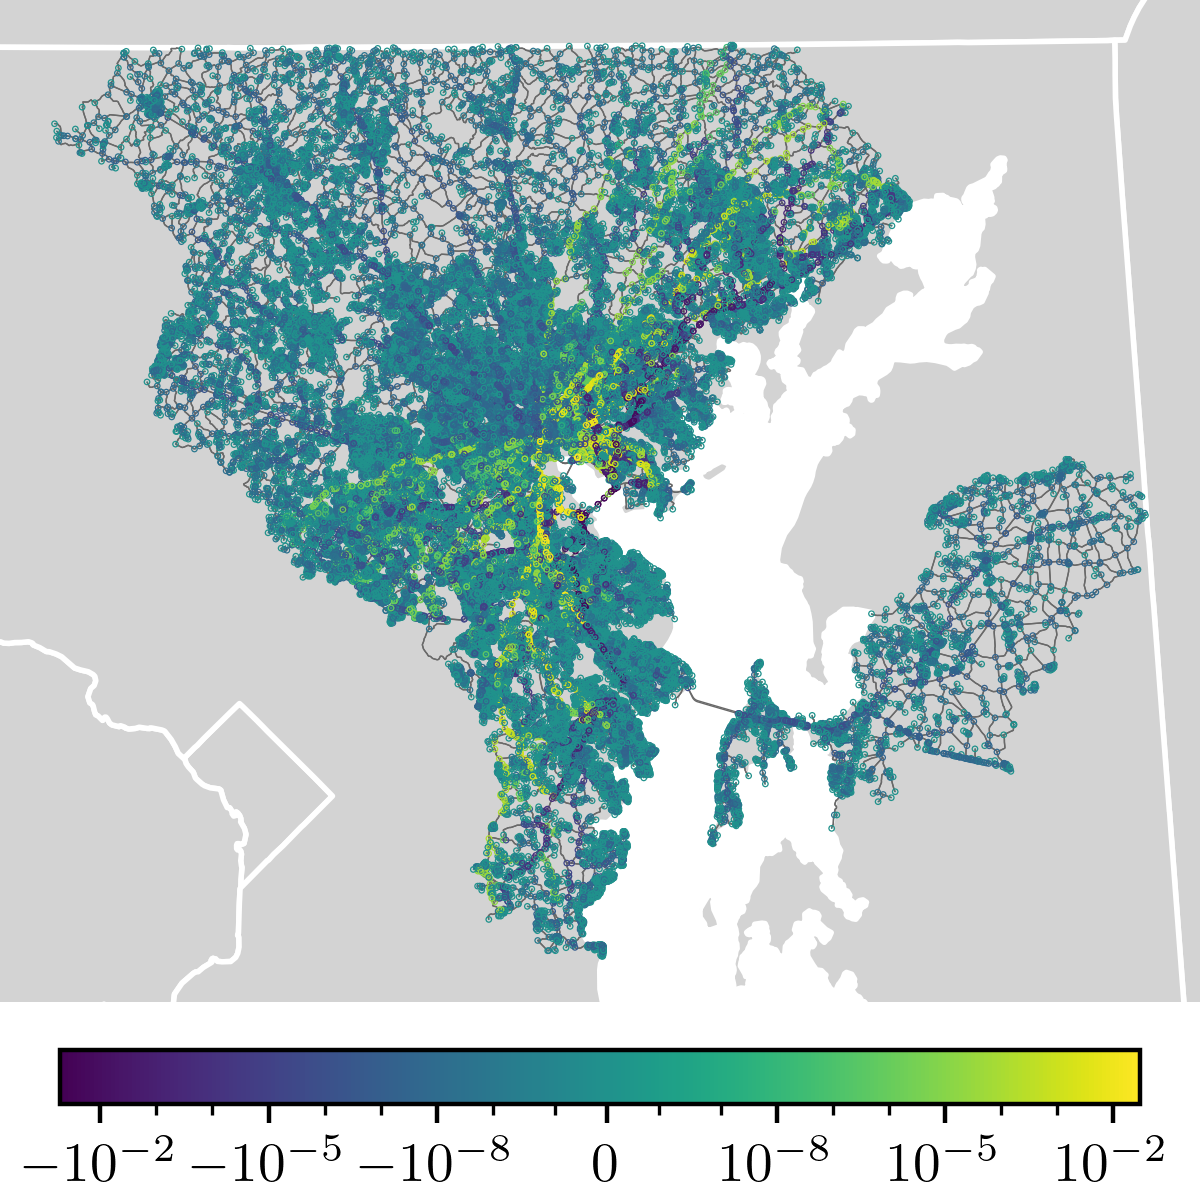
\includegraphics[width=0.28\textwidth]{maps/betweenness_diff.png} \\
      $C^C_i$ & 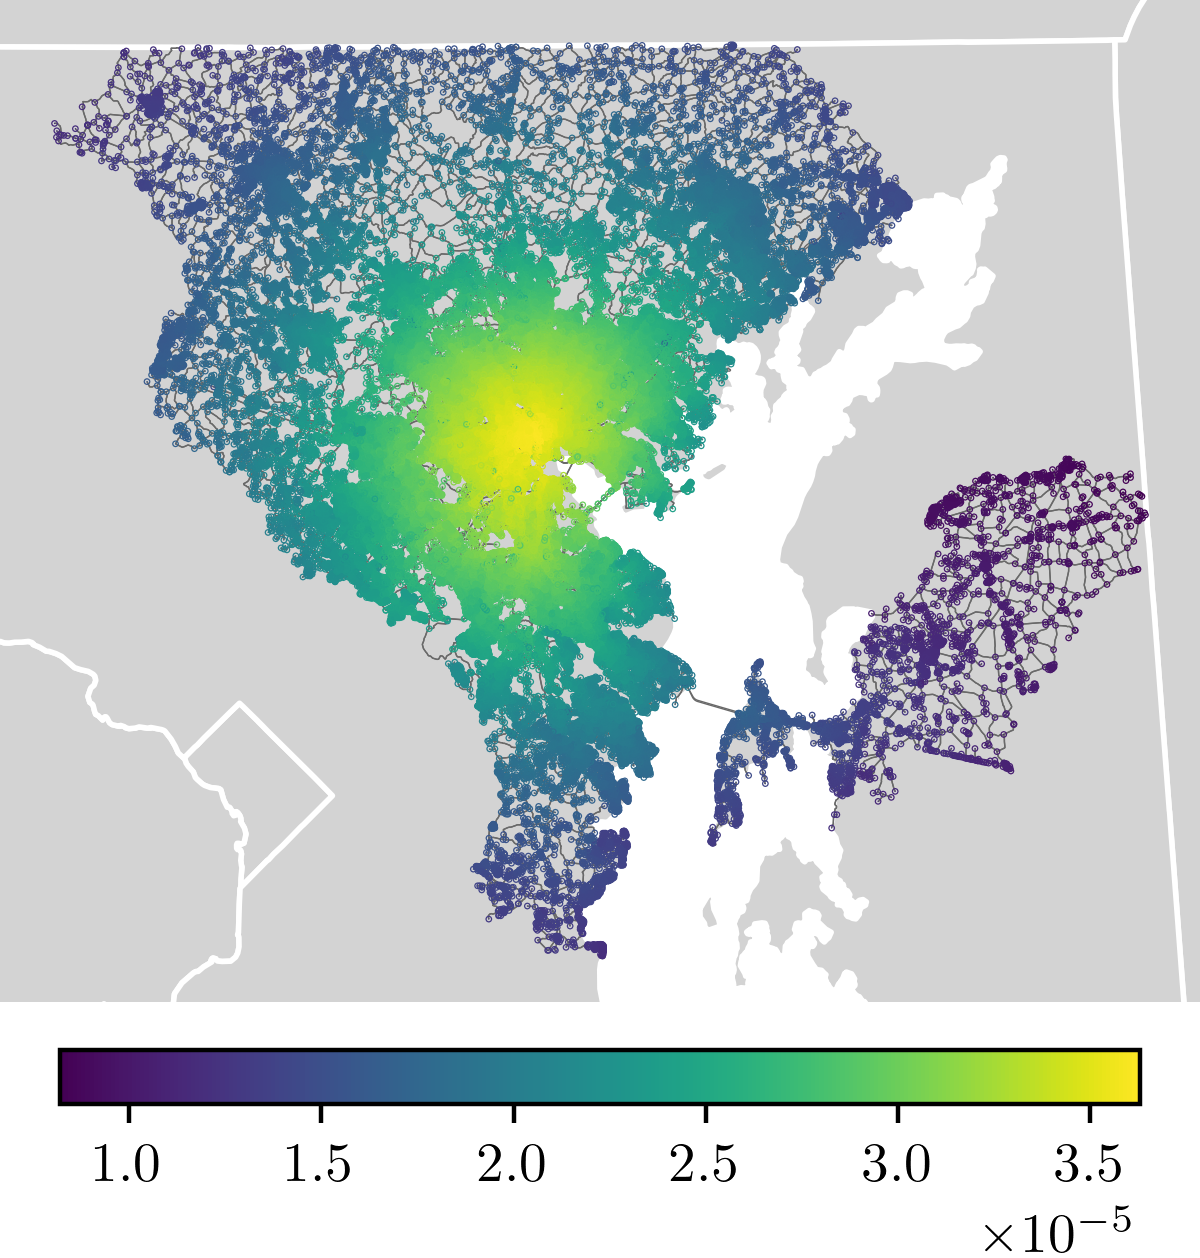
\includegraphics[width=0.28\textwidth]{maps/closeness_w_bridge.png} & 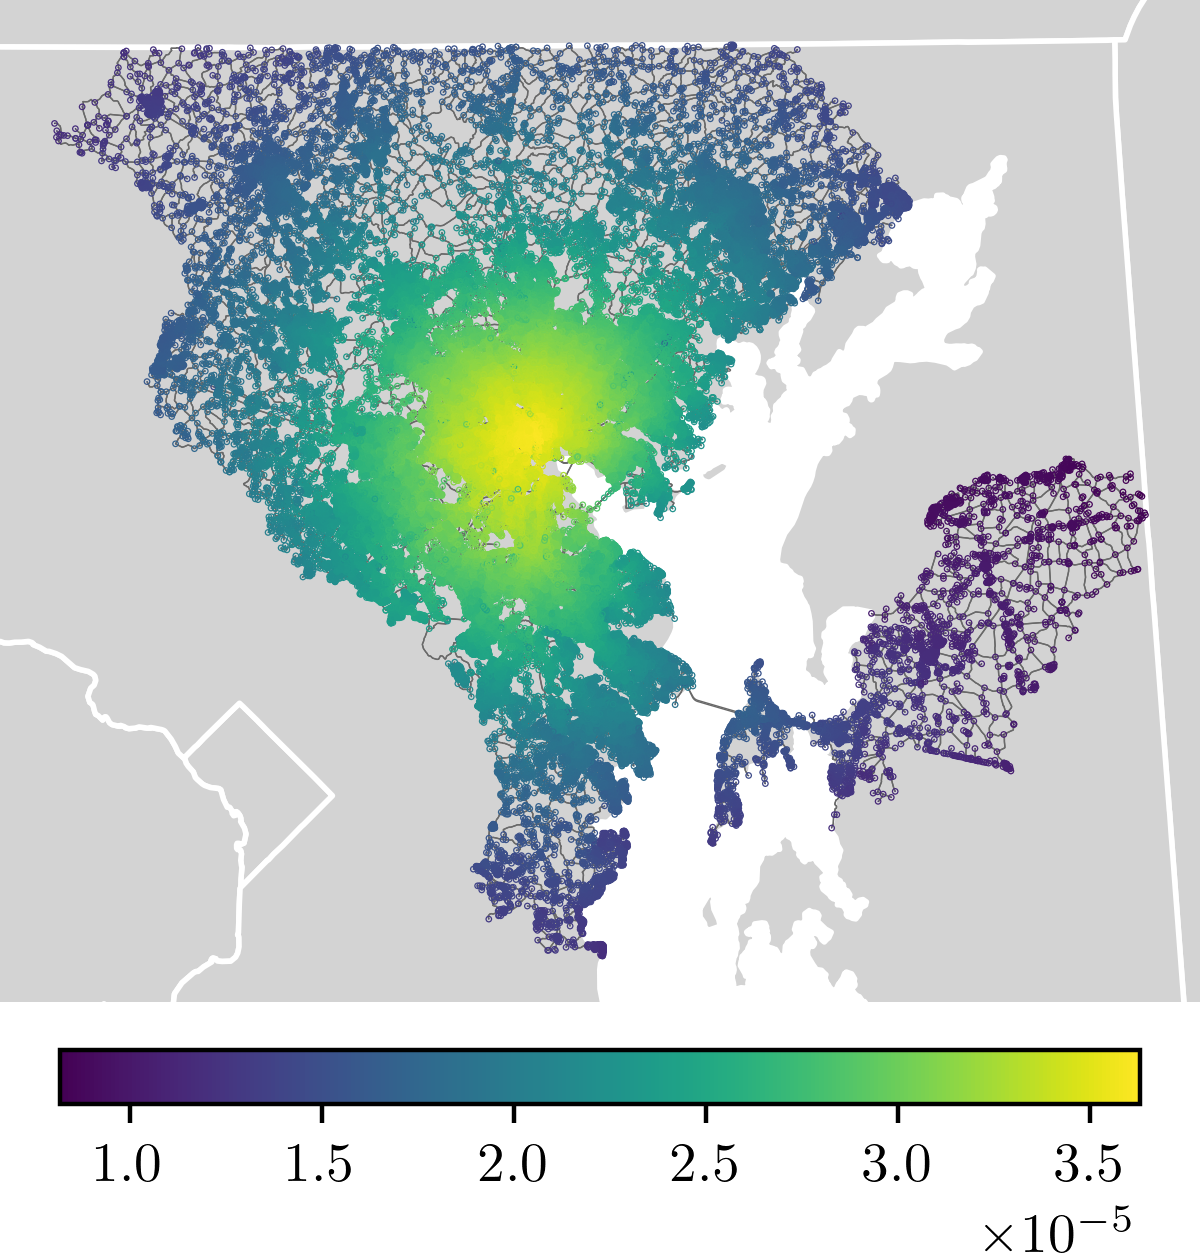
\includegraphics[width=0.28\textwidth]{maps/closeness_wo_bridge.png} & 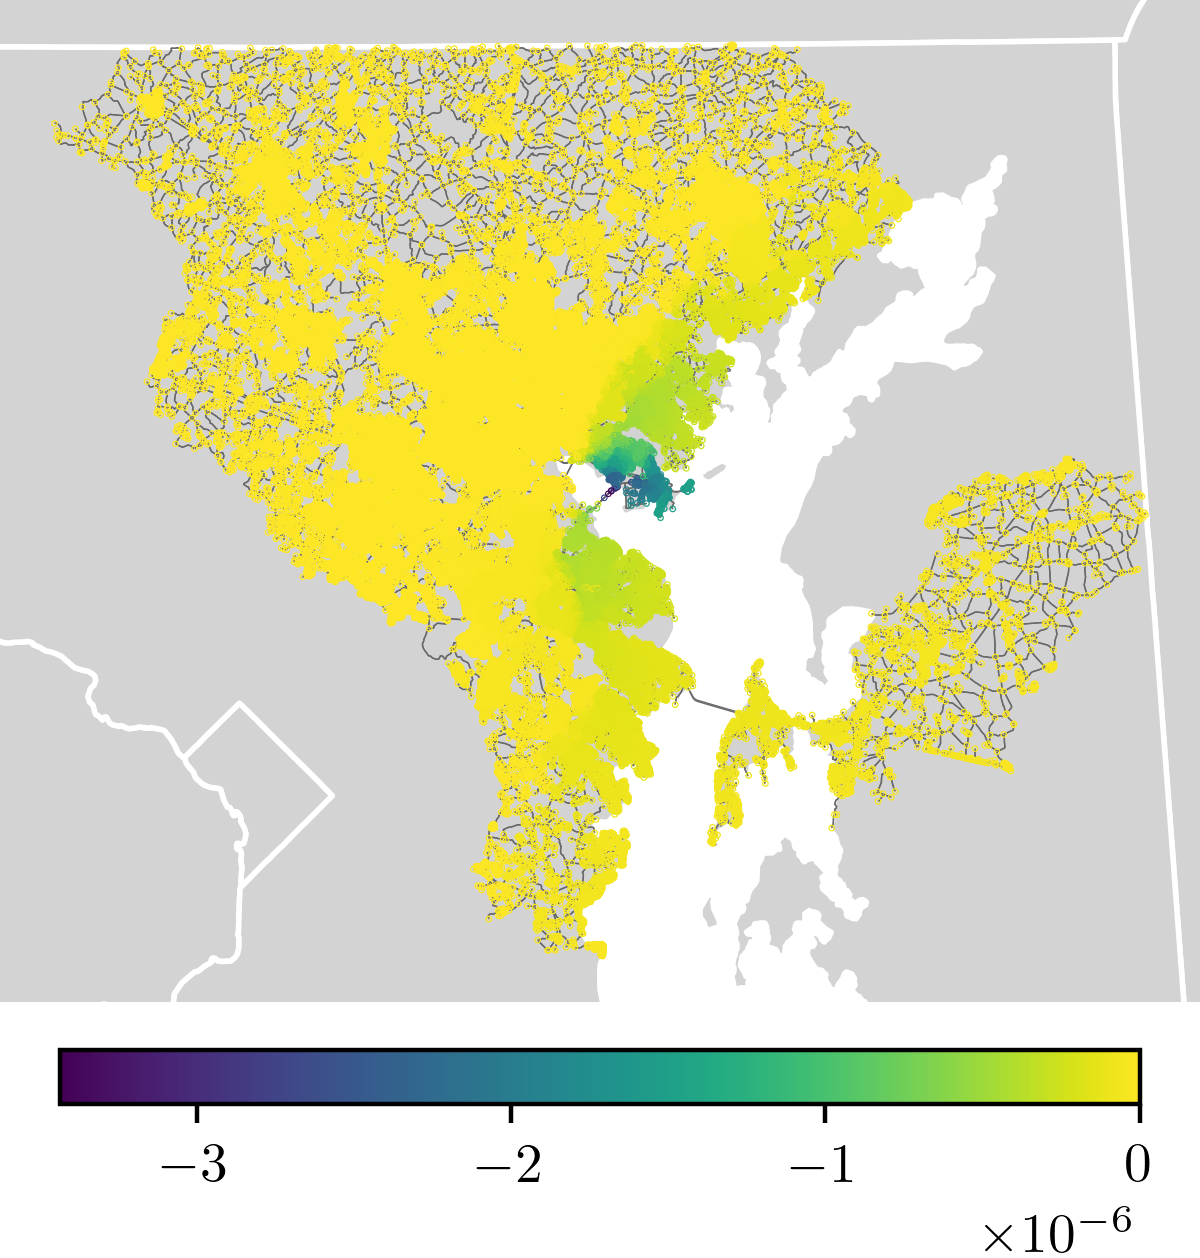
\includegraphics[width=0.28\textwidth]{maps/closeness_diff.png} \\
      $C^S_i$ & 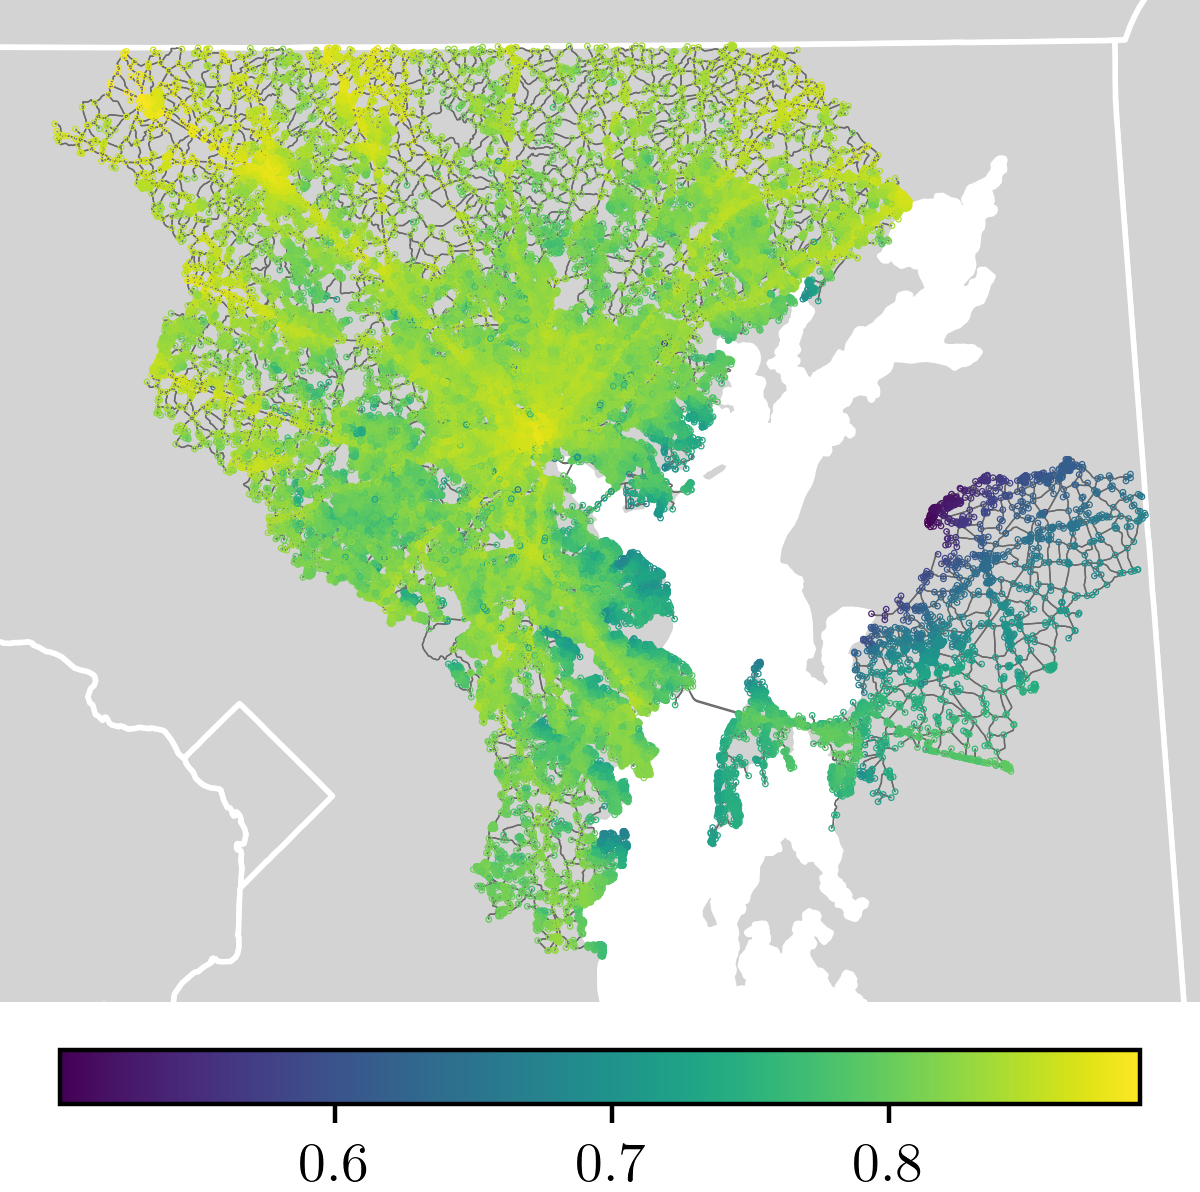
\includegraphics[width=0.28\textwidth]{maps/straightness_w_bridge.png} & 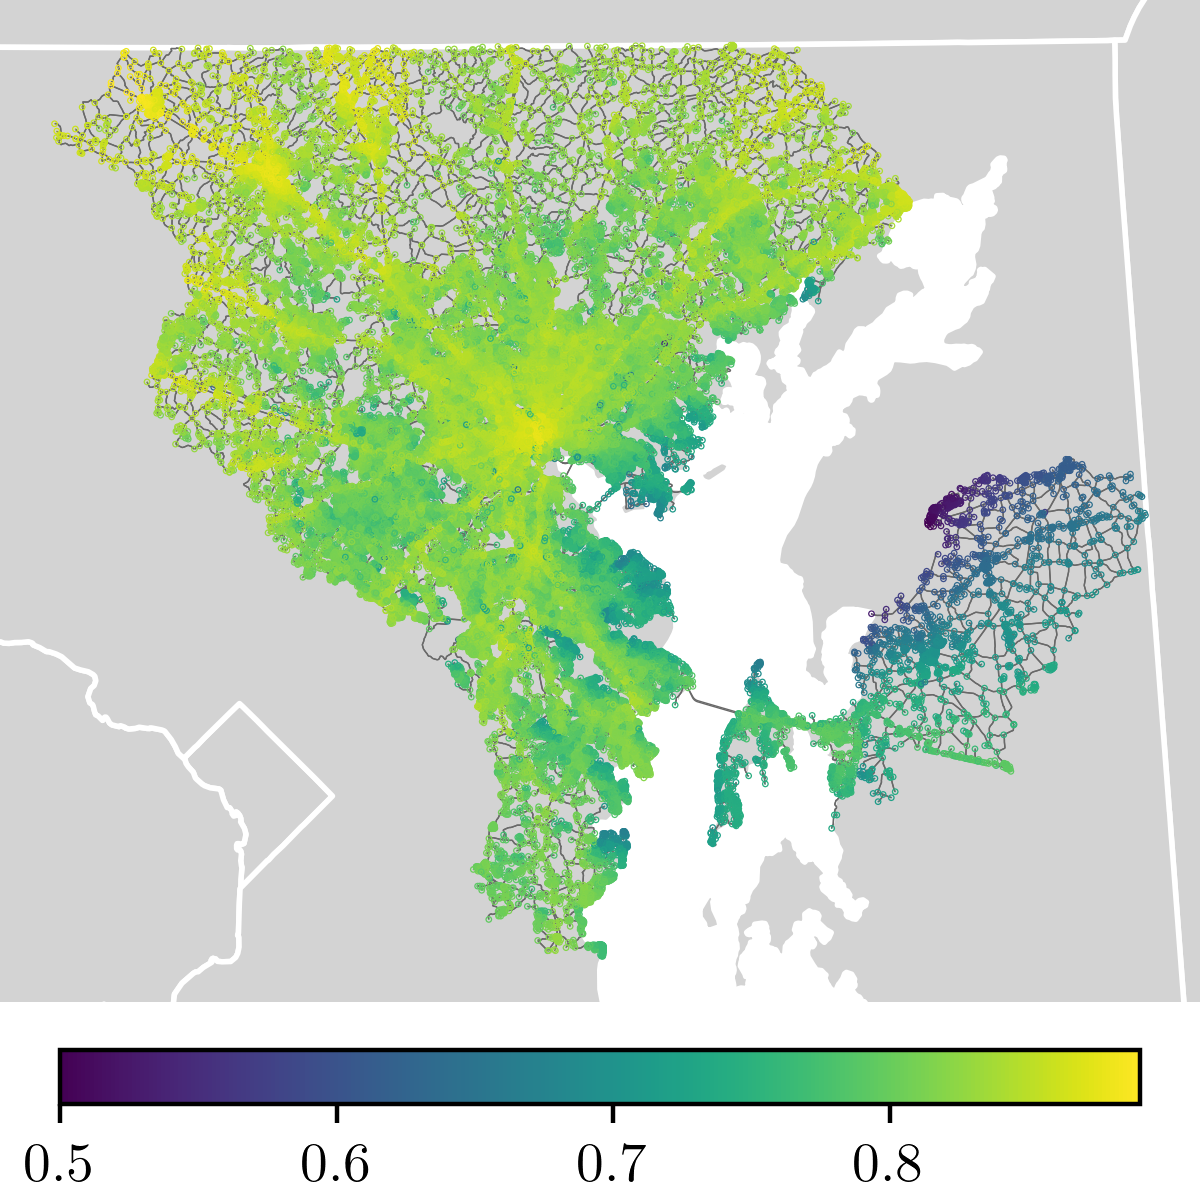
\includegraphics[width=0.28\textwidth]{maps/straightness_wo_bridge.png} & 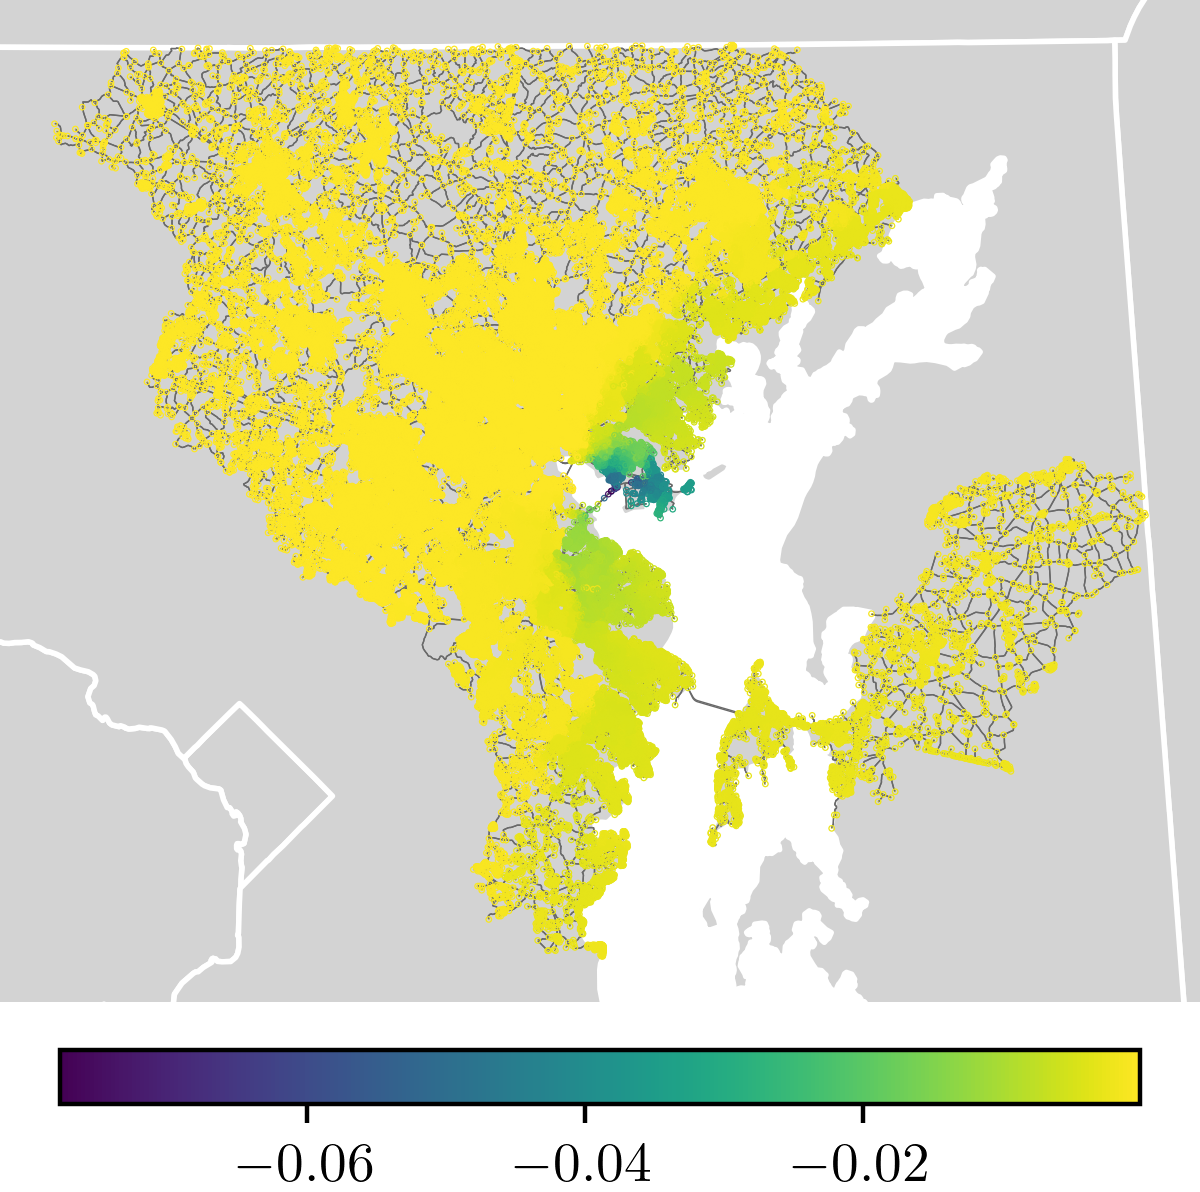
\includegraphics[width=0.28\textwidth]{maps/straightness_diff.png} \\
    \end{tblr}
  } \\
  {\footnotesize Difference calculated a $C_i^\text{Without Bridge} - C_i^\text{With Bridge}$. Log-scale used for Eigenvector and Betweenness centrality and a symmetric log-scale used for their difference. This meant any nodes with 0 weren't plotted, which was between 9,000 and 35,000 nodes depending on the measure. \\}
  \label{fig:cents}
\end{figure}

Both with and without the bridge, the eigenvector centralities are the highest just south of downtown Baltimore. This area has a handful of larger neighborhoods and workplaces (Figure \ref{fig:tracts}) and the BWI airport, consistent with the idea that eigenvector centrality is correlated with areas of high use from \cite{Jayaweera17}.

Without the bridge, the centrality effects are spread throughout the network. The nodes near the bridge are the most affected, but a connected web of nodes that stretches in all directions across the whole network also decreases in centrality. Aside from these specifically affected nodes, nodes generally face a slight increase in centrality, suggesting the importance of the affected nodes was spread throughout the network, though there are a handful of nodes in Queen Anne's county to the east and downtown that face a disproportionate increase in centrality.

The betweenness centrality is highest for nodes at the center of the network and at the ends of bridges, especially the one connecting Queen Anne's county to the east with the rest of the BMA. From these, there are clear paths of high centrality that extend through the rest of the city. Based on \cite{Porta06}, these are likely important paths that are frequently used to traverse the network.

Before it collapsed, the nodes along the Key Bridge were all very important, and paths of other important nodes extended from it, especially along the shore. After the collapse, these nodes became much less important, shown in the path of purple nodes on the difference graph that crosses the bridge and stretches up and down the coast. Instead, paths of increased centrality extend from the Fort McHenry Tunnel (I-95) and the Harbor Tunnel (I-895), which cross the port slightly farther inland than the Key Bridge, and from downtown, which sits at the end of the port.

The closeness centrality both with and without the bridge is centered around the downtown area, likely because it sits at the center of the network. From here, it gradually decreases, and is lowest in corners of the city, especially in Queen Anne's county to the east. This highlights the problems with using closeness centrality on a subset of a network, since the inclusion of other counties surrounding the BMA would likely change where this center of mass sits. Still, the change in the closeness centrality will still be a meaningful indicator of the network implications of the bridge collapse, since nodes are all located in the same place relative to the boundary of our network before and after the event, meaning the bias from this boundary effect should be equivalent on both networks.

The effects of the bridge collapse are almost entirely concentrated near the end of the bridge toward the bay. This makes sense, since, like we saw with the minimal change in average shortest path, nodes aren't that much farther from each other in general, which suggests there should be a minimal change in the closeness centrality for most nodes. The nodes that were affected, however, now have to take a much longer route around the port to get to nodes on the other side, when before they would have just taken the bridge. The nodes to the north were especially affected, likely because routes from them to the south across the port now need to start going north in the wrong direction to get around the port.

The straightness centrality is fairly uniform across both graphs, except in areas where water makes it hard to get to a large portion of the network. This is especially apparent for Queen Anne's county, where the lowest straightness nodes are. Within the rest of the network, there are paths with slightly higher straightness extending out from the center, suggesting these might be either important routes for traversing the network or important areas within the network \parencites{Porta06}{Wang11}.

Like closeness centrality, the effects of the event on straightness centrality are almost entirely concentrated in nodes near the event, especially to the north. The rationale behind this effect is the same: paths that previously would have taken the bridge now have to take a much less direct route around the port, making their path less straight.

Importantly, the bridge collapse didn't benefit the closeness or straightness for any intersections in the network. This makes sense --- the shortest path can't ever be made shorter by removing an edge from the network --- but does contrast the other two centralities where there are winning and losing nodes.

Altogether, our MCA analysis suggests that the effects of the bridge collapse on the ability to travel from a node across the network are concentrated closer to the event, but more dispersed effects are seen in the specific paths taken, affecting traffic through would-be-unaffected intersections.

To analyze the affected paths, we'll focus on the 475 million paths that were impacted, roughly 0.57\% of the possible paths in the total network. This is done both for tractability reasons, there are more than 80 billion node-to-node paths in the network as a whole which would pose significant problems for computability, and analysis reasons, since the effect of these 99.43\% of paths that are unaffected is seen in the minuscule change in the average shortest path length. Summary statistics for this distribution are shown in Table \ref{tab:spaths}. The mean and standard deviation are similar, evidencing the wide spread of the distribution. The mean is larger than the median, which suggests there is a right skew. The distribution and geographic start points of these shortest paths are shown in Figure \ref{fig:spaths}.

\begin{table}[t!]
  \caption{Summary statistics for the difference in affected paths (miles).}
  \centering
  \begin{tabular}{cccccccc}
    \toprule
    \textbf{Count} & \textbf{Mean}& \textbf{St. Dev.} & \textbf{Min} & \textbf{25\%} & \textbf{Median} & \textbf{75\%} & \textbf{Max} \\
    \midrule
    $4.750 \times 10^8$ & 1.525 & 1.514 & $1.864 \times 10^{-6}$ & 0.559 & 1.049 & 2.018 & 15.716 \\
    \bottomrule
  \end{tabular}
  \label{tab:spaths}
\end{table}

\begin{figure}[t!]
	\caption{Changes in shortest paths}
  \begin{subfigure}{0.49\textwidth}
    \centering
    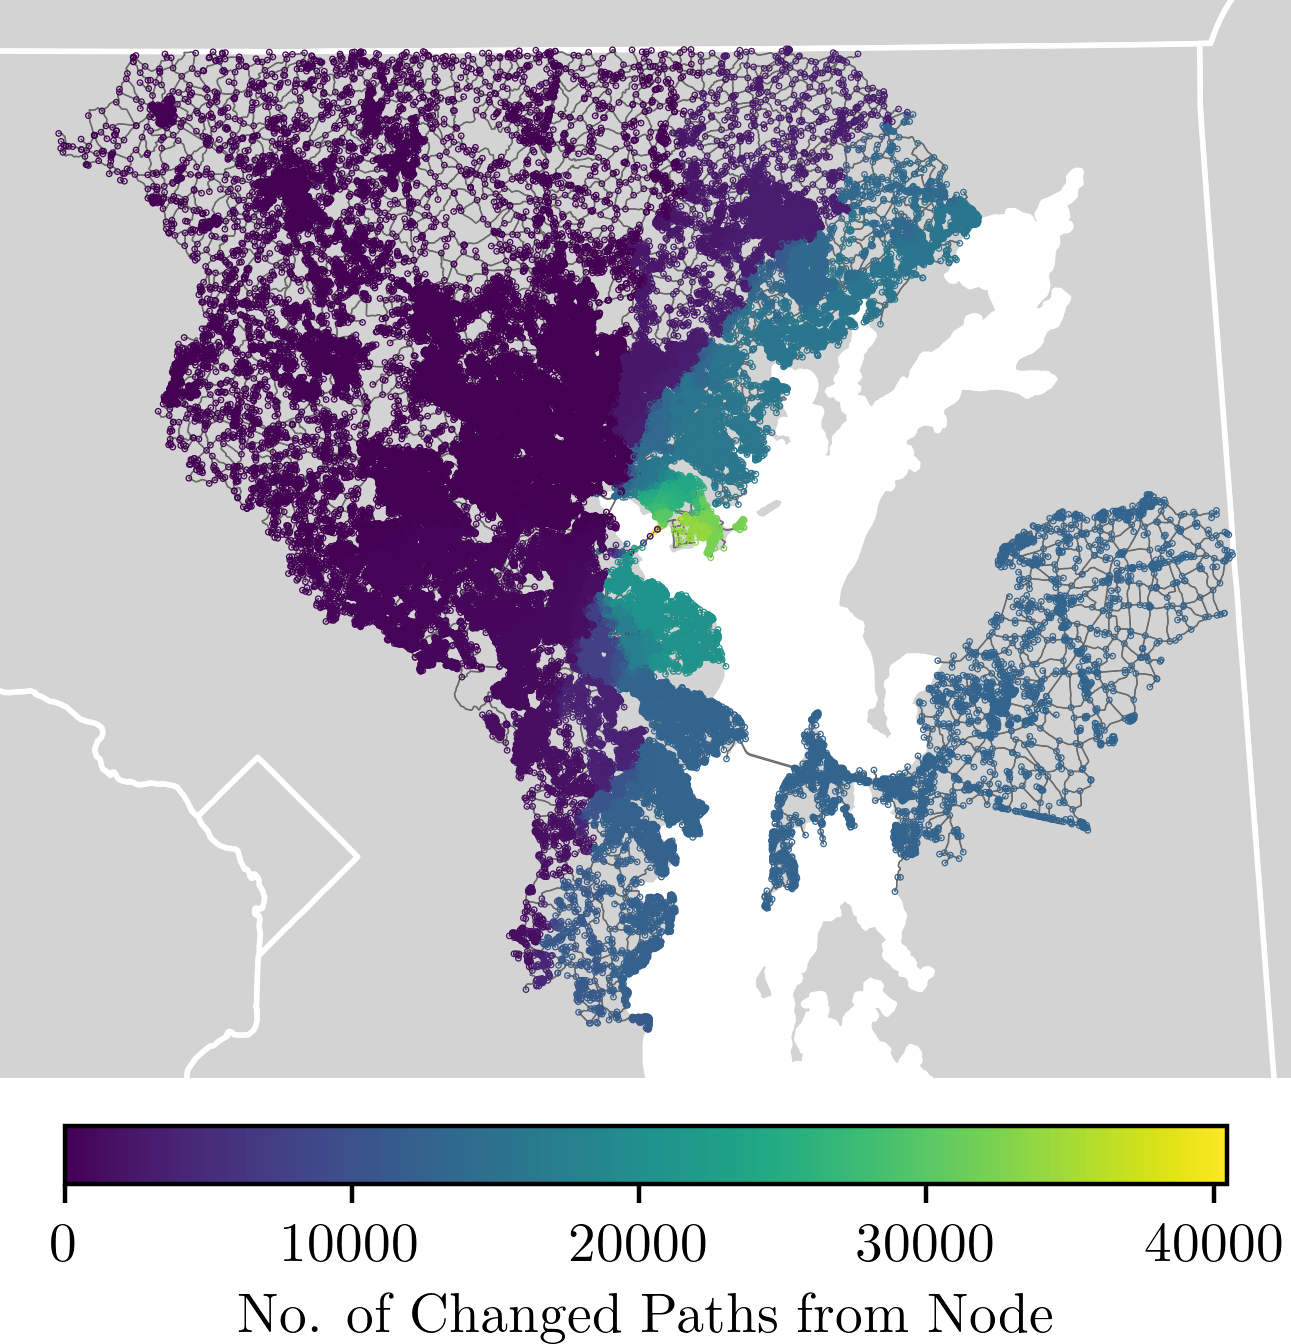
\includegraphics[width=\textwidth]{maps/no_changed_paths.png}
    \caption{Total Number of Longer Shortest Paths Starting at Each Node}
  \end{subfigure}
  \begin{subfigure}{0.49\textwidth}
    \centering
    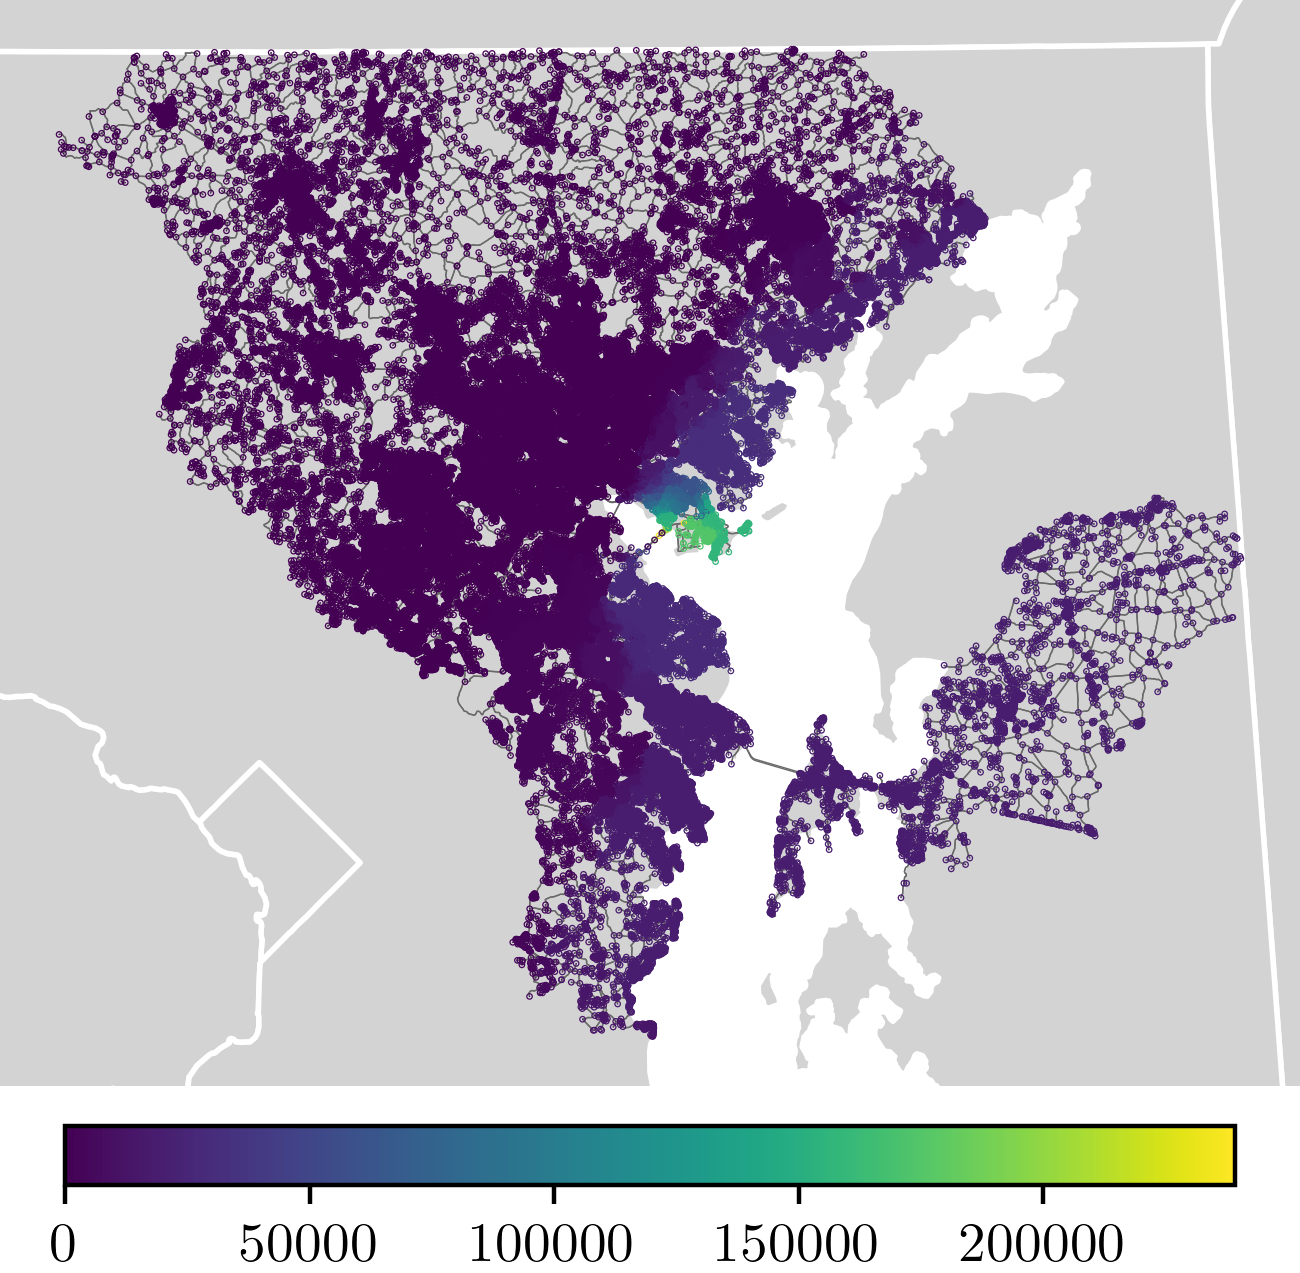
\includegraphics[width=\textwidth]{maps/dist_changed_paths.png}
    \caption{Total Difference in Distance for All Shortest Paths Starting at Each Node (Miles)}
  \end{subfigure}
  \begin{subfigure}{\textwidth}
    \centering
    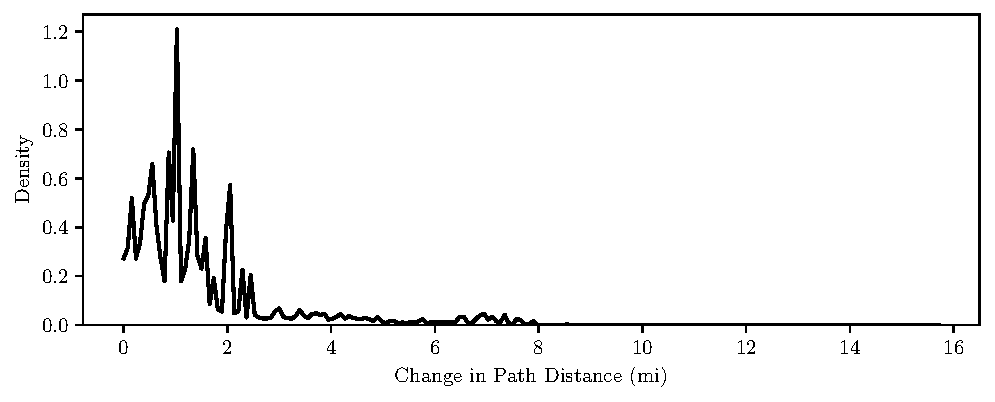
\includegraphics[width=\textwidth]{graphs/path_dists.pdf}
    \caption{Difference in Distance Traveled Along Path (Miles)}
  \end{subfigure}

  \label{fig:spaths}
\end{figure}

The maps show that nodes all along the coast had significant numbers of paths that would have gone over the bridge and were affected, but these only significantly affect travel distances closer to the bridge and the port, since by cutting in at a slight angle someone traveling from farther north or south can get around the port without using the bridge and adding little distance to their route, while someone traveling from closer has to cut straight west first.

Like we saw from the summary statistics, the distribution of path distances has a strong right skew and a lot of noise. This means that most affected paths weren't lengthened significantly, but a handful of paths were, which means the impacts of the bridge collapse are localized to people traveling a handful of routes and not necessarily felt by everyone in the BMA area.


\subsection{Network Utilization}

Based on our utilization weighted model, the average commute to work is 11.43 mi (18.39 km) before the bridge collapsed and 11.44 mi (18.40 km) after. This is less than half of the average shortest path along the network, and points to the idea that people are choosing to live and work closer together than would be expected if both choices were independent, meaning that our structural analysis might overweight long trips. The bridge collapse caused the average commute distance to increase by 0.010 miles or 0.016 km, more than we predicted without weighting by use, but still a fairly insignificant amount.

For our centrality measures, two of them, closeness and straightness, require flow originating at the node, meaning we can only find them at a tract level, while the other one, betweenness, is still meaningful at a node-level. These statistics are shown in Figure \ref{fig:use_cents}.

\begin{figure}[t!]
  \caption{Node centrality before and after the bridge collapse.}
  \centering
  \begin{tblr}{%
    colspec = {cX[c,h]X[c,h]X[c,h]},
    rowsep = 0pt,
    colsep = 4pt
    }
    & \textbf{Network With Bridge} & \textbf{Network Without Bridge} & \textbf{Difference} \\
    $C^B_i$ & 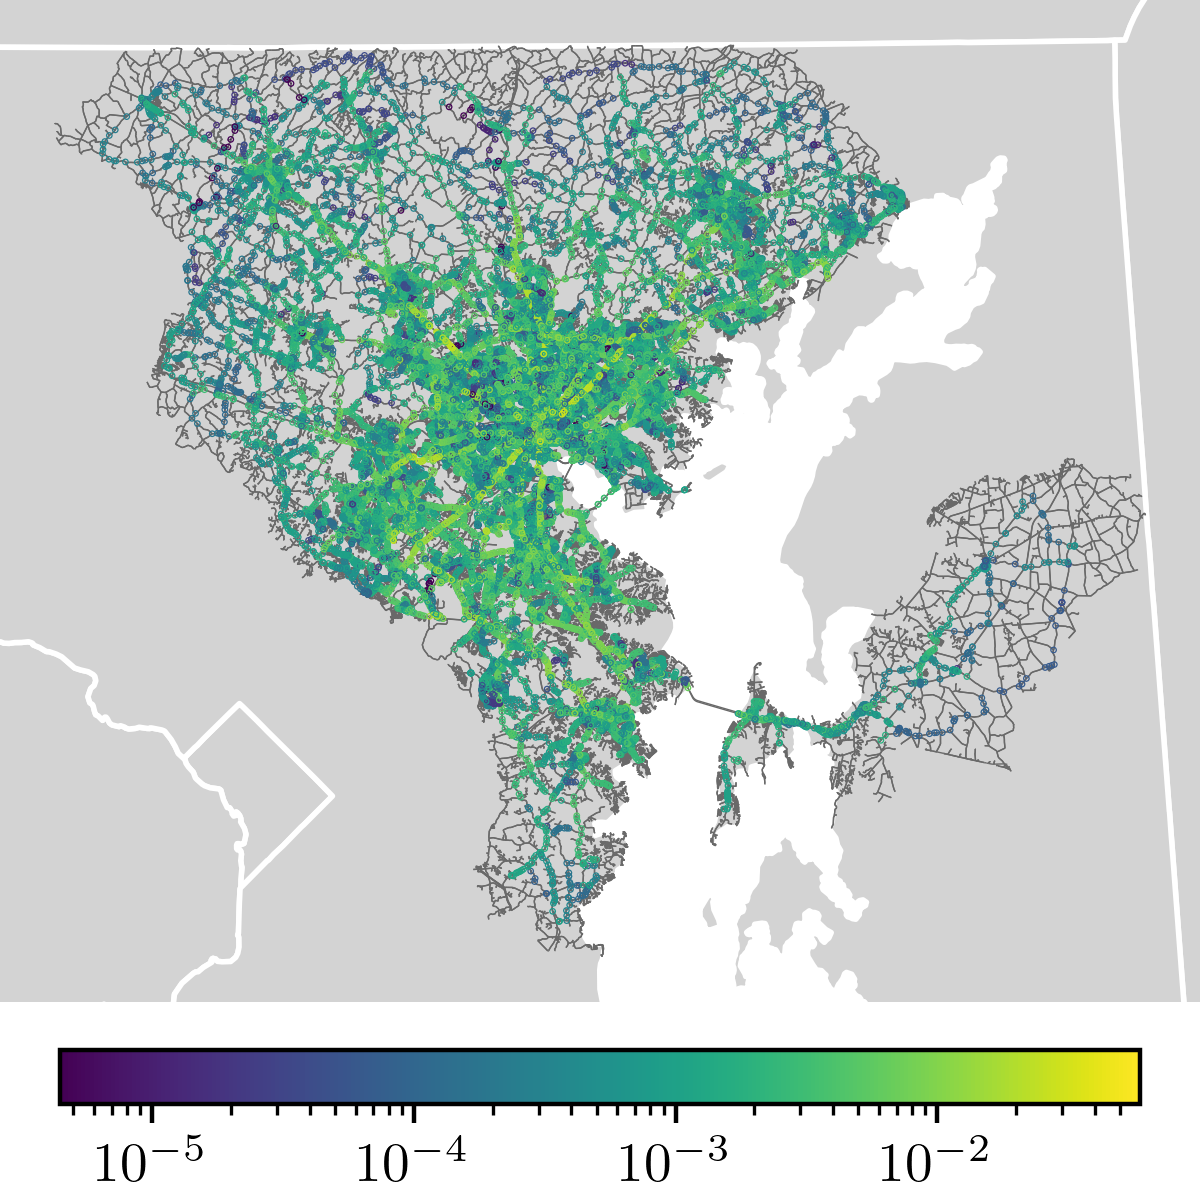
\includegraphics[width=0.28\textwidth]{maps/use_betweenness_w_bridge.png} & 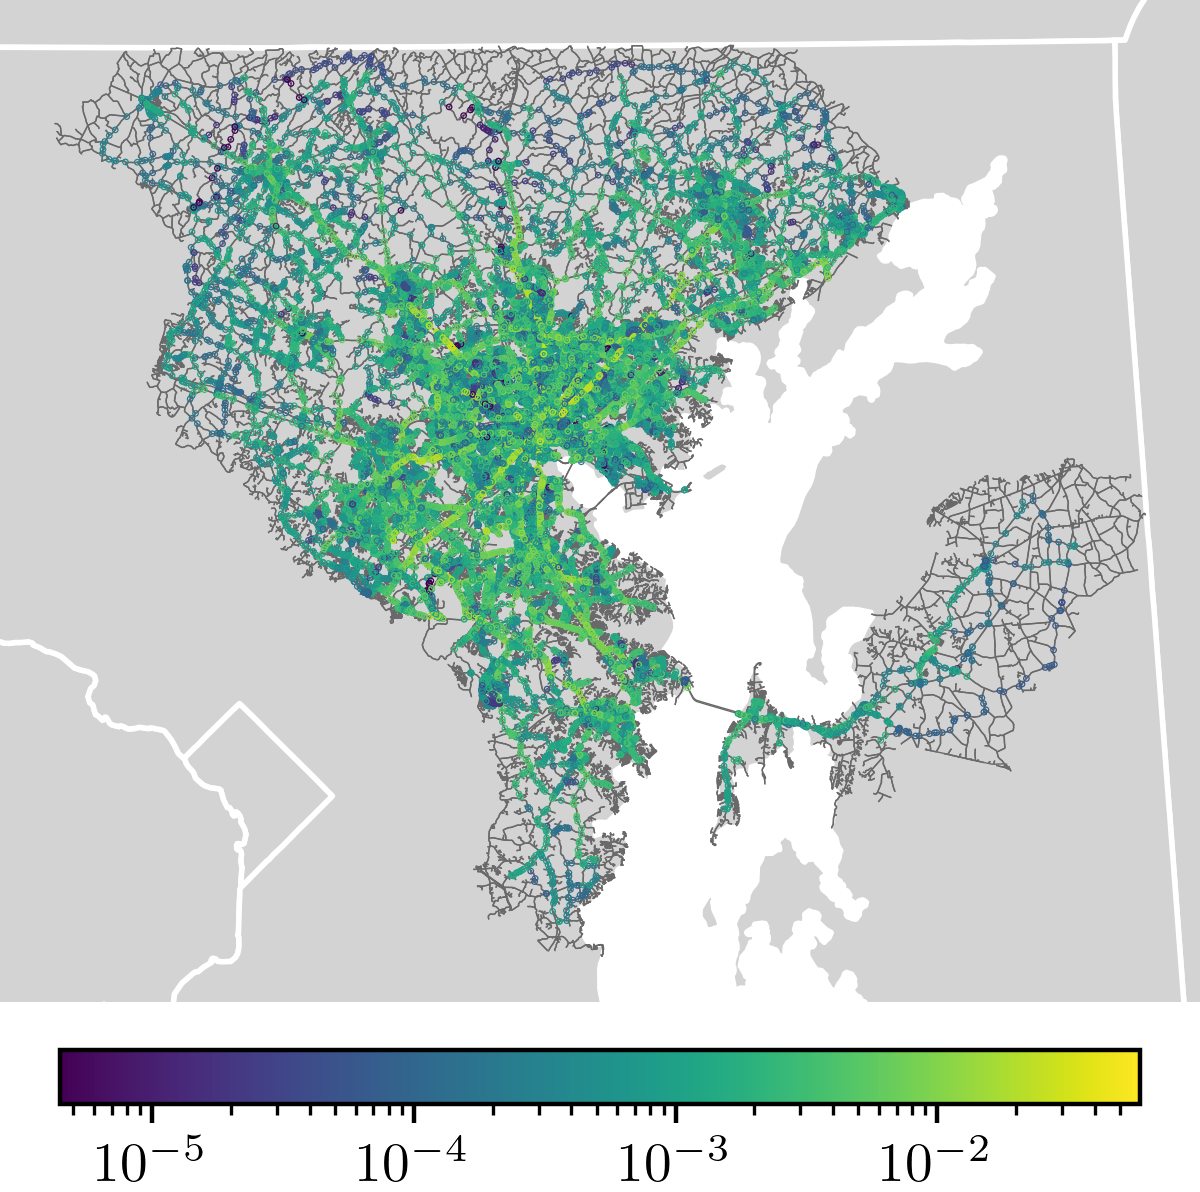
\includegraphics[width=0.28\textwidth]{maps/use_betweenness_wo_bridge.png} & 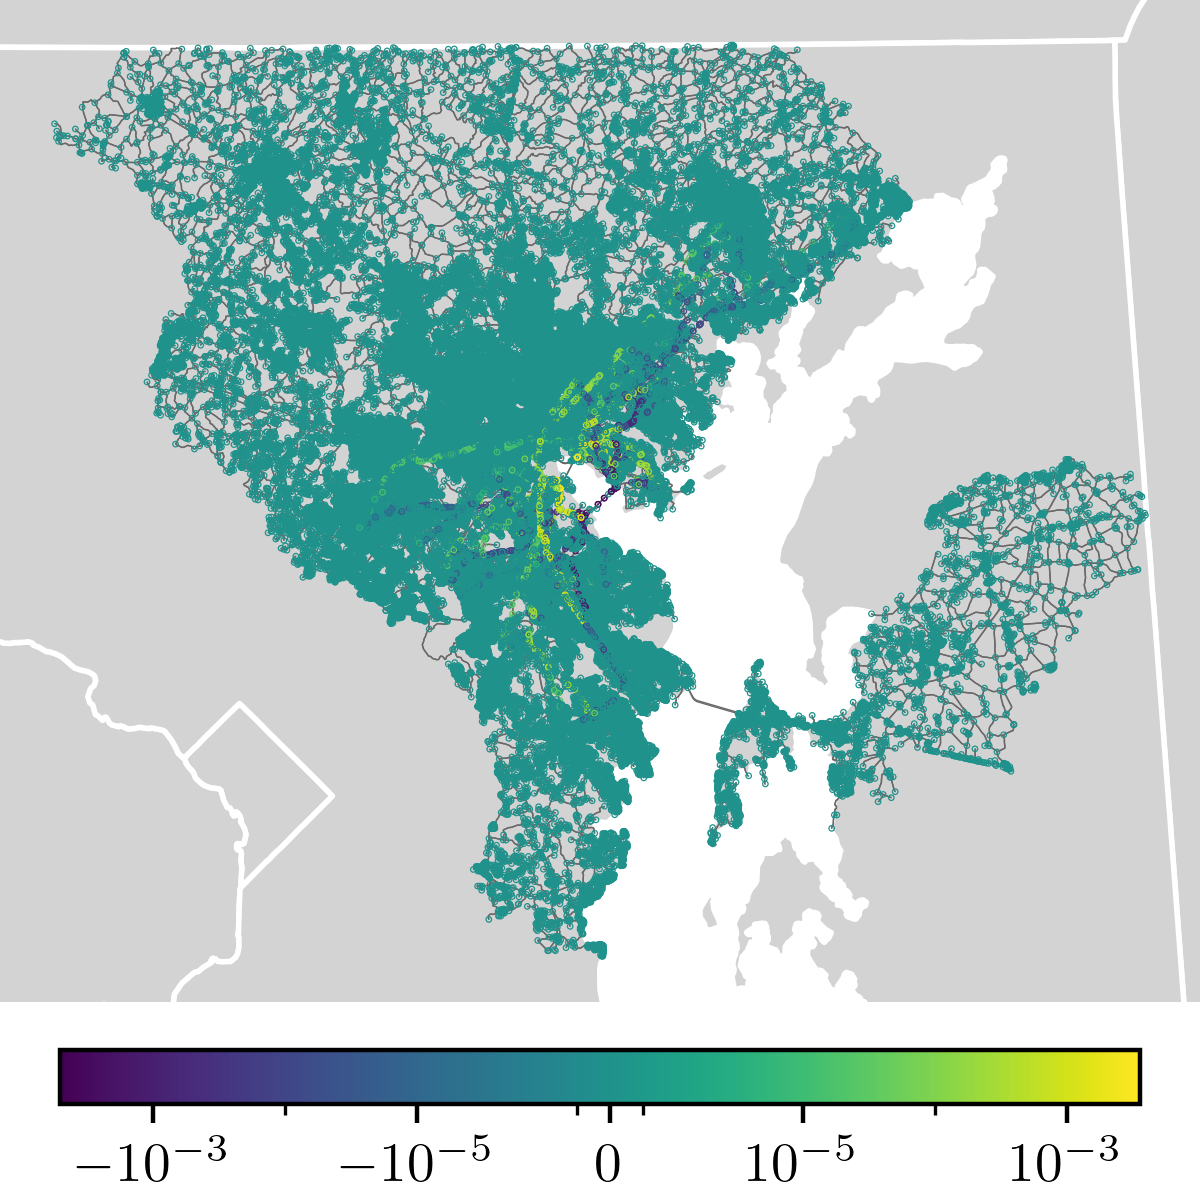
\includegraphics[width=0.28\textwidth]{maps/use_betweenness_diff.png} \\
    $C^C_i$ & 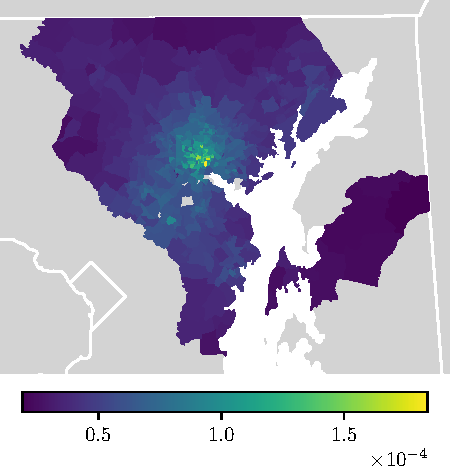
\includegraphics[width=0.28\textwidth]{maps/use_closeness_w_bridge.pdf} & 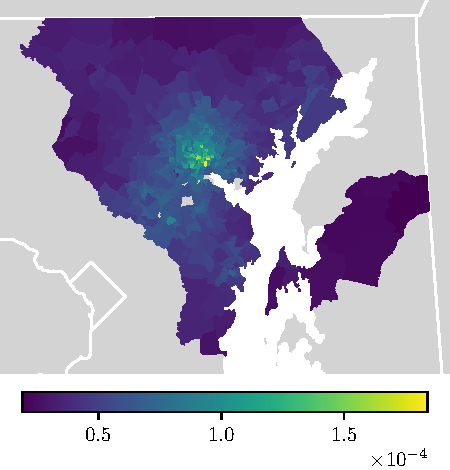
\includegraphics[width=0.28\textwidth]{maps/use_closeness_wo_bridge.pdf} & 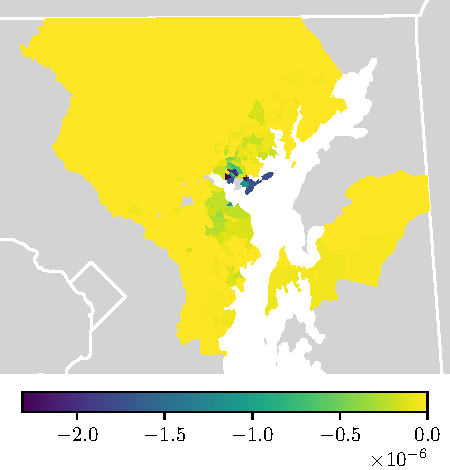
\includegraphics[width=0.28\textwidth]{maps/use_closeness_diff.pdf} \\
    $C^S_i$ & 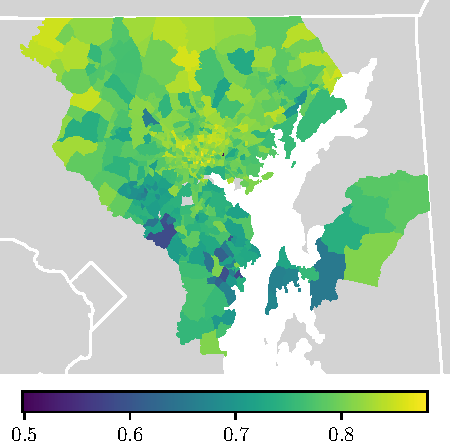
\includegraphics[width=0.28\textwidth]{maps/use_straightness_w_bridge.pdf} & 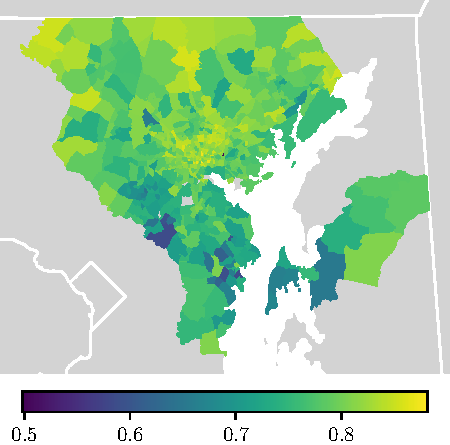
\includegraphics[width=0.28\textwidth]{maps/use_straightness_wo_bridge.pdf} & 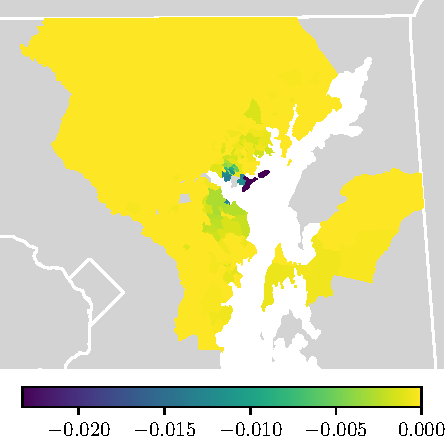
\includegraphics[width=0.28\textwidth]{maps/use_straightness_diff.pdf} \\
  \end{tblr}
  {\footnotesize Difference calculated a $C_i^\text{Without Bridge} - C_i^\text{With Bridge}$. Log-scale used for Betweenness centrality and a symmetric log-scale used for its difference. This meant approximately 57,000 nodes with 0 centrality weren't plotted. \\}
  \label{fig:use_cents}
\end{figure}

As expected by excluding most nodes as possible origin points, there are quite a few more nodes with 0 betweennesses, making the network more sparse. Still, we see similar patterns as the standard betweenness centrality since high-betweenness paths extend from high-betweenness nodes in the center and near bridges, likely representing important routes in the overall road network.

The effects of the bridge collapse are much more pronounced on the nodes they affect, but affect fewer nodes. In Figure \ref{fig:cents}, there are faint routes of different centrality that span the whole network, but here only specific routes, namely along the coast are affected, but this difference is much more stark.

Closeness centrality is, again, concentrated around the center, though it tapers off much more quickly. This could be caused by people who live downtown valuing living and working closer together more than those that live in other parts of the city or the suburbs, causing them to be closer to where they work.

The effects of the bridge collapse are even more localized when accounting for use than without. In Figure \ref{fig:cents}, the effects of the collapse can be seen in a wide range of nodes near the bridge, but when accounting for use only a small area to the north of the bridge is affected. The couple tracts that are affected, however, see an impact that's similar in magnitude to before. This suggests only a couple tracts near the bridge have a significant amount of people cross the bridge in their commute.

The use-weighted straightness centrality exhibits far more variability than before. In Figure \ref{fig:cents}, there is limited difference between nodes within geographic areas, but the variability between geographic areas is far more significant. Here, much of the variability between geographic areas goes away, possibly because people are working near where they live, but straightness within nearby tracts in geographic areas varies significantly more.

Like with closeness, the effects of the collapse are very localized to the area just north of the port near the bridge relative to the network-wide estimations in Figure \ref{fig:cents}. Again, this suggests that only a handful of tracts are home to significant numbers of commuters that used the bridge.

Altogether, our use based analysis suggests that the effects of the collapse are still significant, but very localized to commuters that live in certain areas and that the traffic going through intersections is only affected in a handful of routes, not in a web that spans the network like we found without using use-weighted statistics.


\section{Conclusion} \label{sec:concl}

Through our network analysis of the Key Bridge collapse, we found significant local impacts but limited global impacts from the event. On average, paths across the network only increase slightly in length. However, in specific areas, especially near the bridge, we see significant impacts. This is evident in the change in closeness and straightness centrality, especially when weighted by use where the impacts become even more localized than would be suggested in an analysis of the network as a whole. The betweenness and eigenvector centralities suggest that the implications of the blockage will propagate and affect traffic and importance for intersections in a web throughout the network, especially along the coast. The origins of affected path lengths also suggest a very localized effect, and the right-skew of the distribution suggests that only specific paths are the most impacted.

The results of our analysis, especially in regard to betweenness centrality, are very consistent with behavior patterns we're observing after the collapse. The Fort McHenry Tunnel and Harbor Tunnel, which we predicted would increase in betweenness due to the event, have experienced a significant increase in traffic after the event \parencite{Domen24}. This consistency with the real world suggests the use of this type of network analysis to examine the road network is valuable and paints an accurate picture of the implications of the event.


\subsection{Limitations}

Our analysis has a handful of limitations. Mostly because of the small size of the shock to the network (one edge), we don't examine the change in the size of the largest connected component, the clustering coefficients, or modularity classes and community divisions, factors which are often used in the literature to analyze road network shocks \parencites{Xeumei10}. These weren't affected by the removal of a single bridge, so analysis of them that's more in line with other network attack literature would be uninformative.

The network itself also has an arbitrary boundary. We chose the network to include all counties in the BMA area, but the BMA road network isn't completely disconnected from that of the rest of Maryland and United States. In that way, our analysis might not be able to analyze how far the collapse effects propagate. Intersections with affected betweenness centrality extended all the way to the north and south of the network and don't taper off within our bounds, but this pattern could change if the network size was larger. Due to the boundary, our use analysis also ignores the significant number of paths that travel between the BMA area and the surrounding counties.

Our analysis of the tract-to-tract commuter flow data also has a handful of limitations. It relies on a couple key assumptions, namely that everyone travels by car using the road network and starts and ends in the center of their tract, that reflect simplified versions of reality. We also ignore trips that don't go from the home tract to the workplace tract. These ignored trips include commutes home after work, which could be modeled by flipping the start and endpoints in the analysis, and other trips people make by car, like when running errands or exploring the city. Therefore, our analysis should be interpreted in the context of trips people make to work and not general road use.


\subsection{Future Work}

Future work could work on incorporating other use-related data sources, for example average annual daily traffic or work-to-home tract trips, with our network. This would help get a better view of how people's use of the network was affected by the collapse, but, at least for AADT data, isn't feasible until the end of 2024 when these numbers will be released for the time of the collapse. A more empirical analysis that compares network statistics to actual effects would help inform and contextualize future research on the topic, since it would allow researchers to better understand what the differences in network statistics and centrality measures actually mean in a real world context.

Future work could also look more at what types of nodes were impacted. Knowing whether these were highways, arterial roads, or side streets would be valuable and help inform how we interpret the effects of the shock.

\clearpage
\printbibliography

\end{document}